\begin{savequote}[75mm]
   If I model a phenomenon accurately, does that mean I understand it? Or might it be simple coincidence, or an artifact
   of the technique? Of course, as an ardent simulationist, I myself put much faith in Engine-modeling.
\qauthor{Edward Mallory, The Difference Engine by William Gibson and Bruce Sterling}
\end{savequote}

\chapter{Wyniki}


%The following two sections describe
%different non-linear evolution of streaming instability in quasi-global setup
%with reference to similar case shown by JY07.

\section{Symulacje dwuwymiarowe}
Poniżej przedstawiono opis wyników uzyskanych dla symulacji w przypadku
dwuwymiarowym. Ich celem, w połączeniu z liniową analizą stabilności, była
weryfikacja zaimplementowanych metod oraz poprawności przyjętego modelu. Każdy z
przedstawionych wyników można porównać do analogicznych eksperymentów
numerycznych z pracy JY07~\cite{JY07}. Pomimo istotnych różnic w użytych
metodach (JY stosowali kod wysokiego rzędu -- PENCIL, a także traktowali pył
jako cząstki materialne, a nie płyn), wyniki we wszystkich przypadkach wykazują
zgodność ilościową i jakościową.

\subsection{Luźno związane ,,kamienie''}% ($a=50\,\textrm{cm}$, $\tau_s\approx
%1.2$)\label{marg_boulders}}

\begin{figure*}
   \centering
   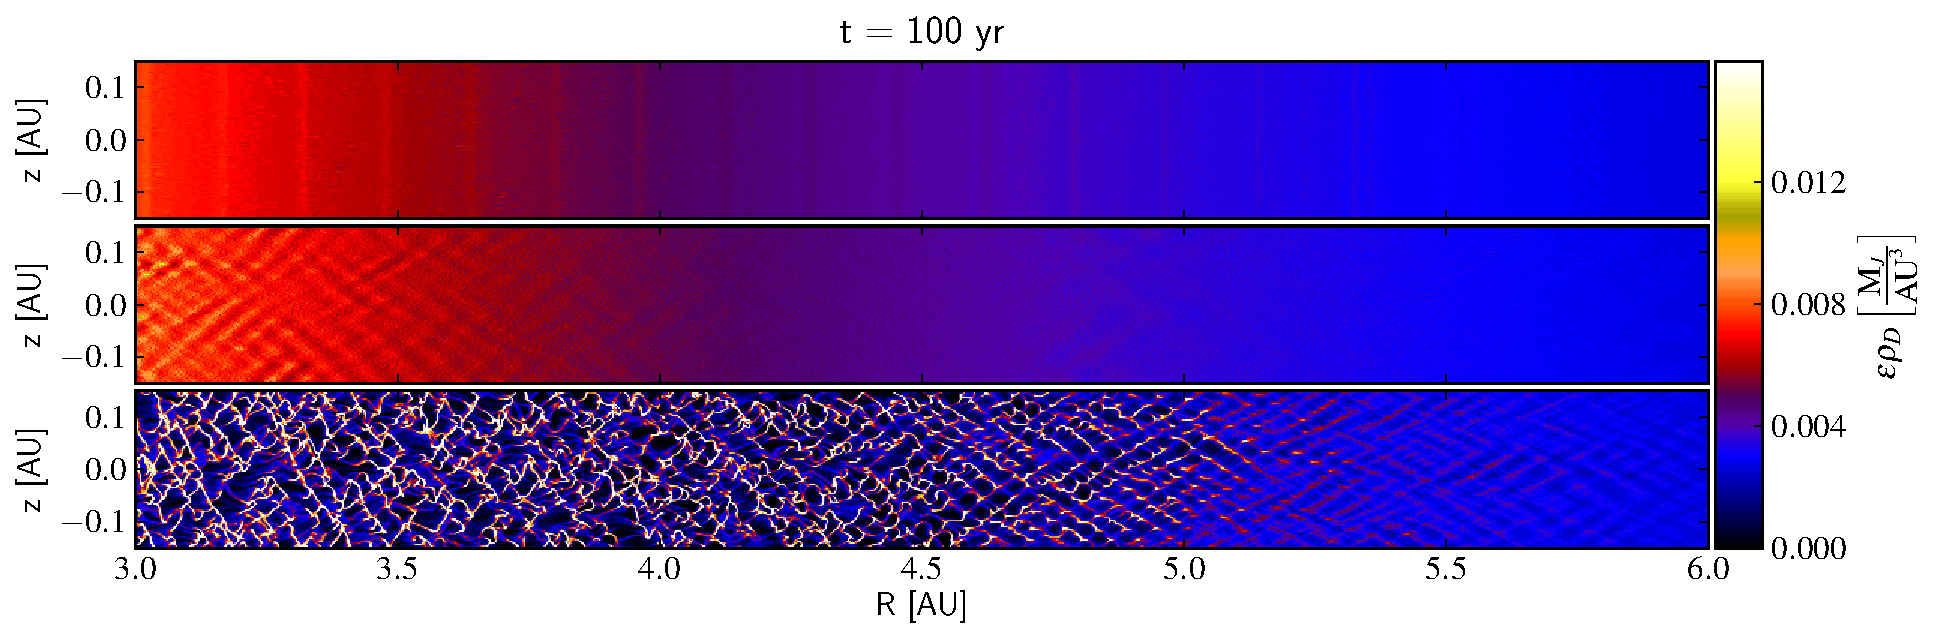
\includegraphics[width=0.99\linewidth]{figures/fig1a}
   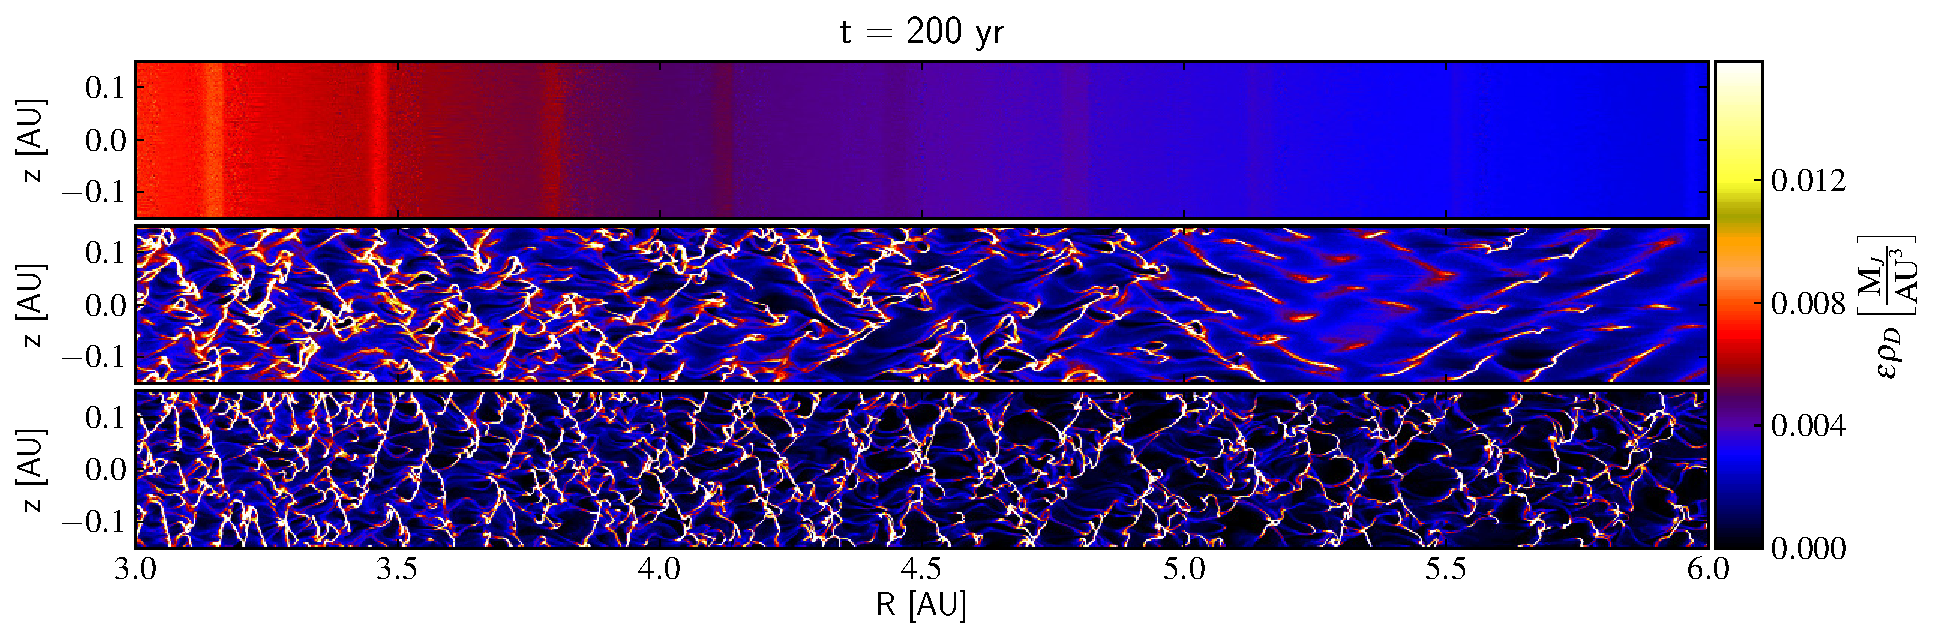
\includegraphics[width=0.99\linewidth]{figures/fig1b}
   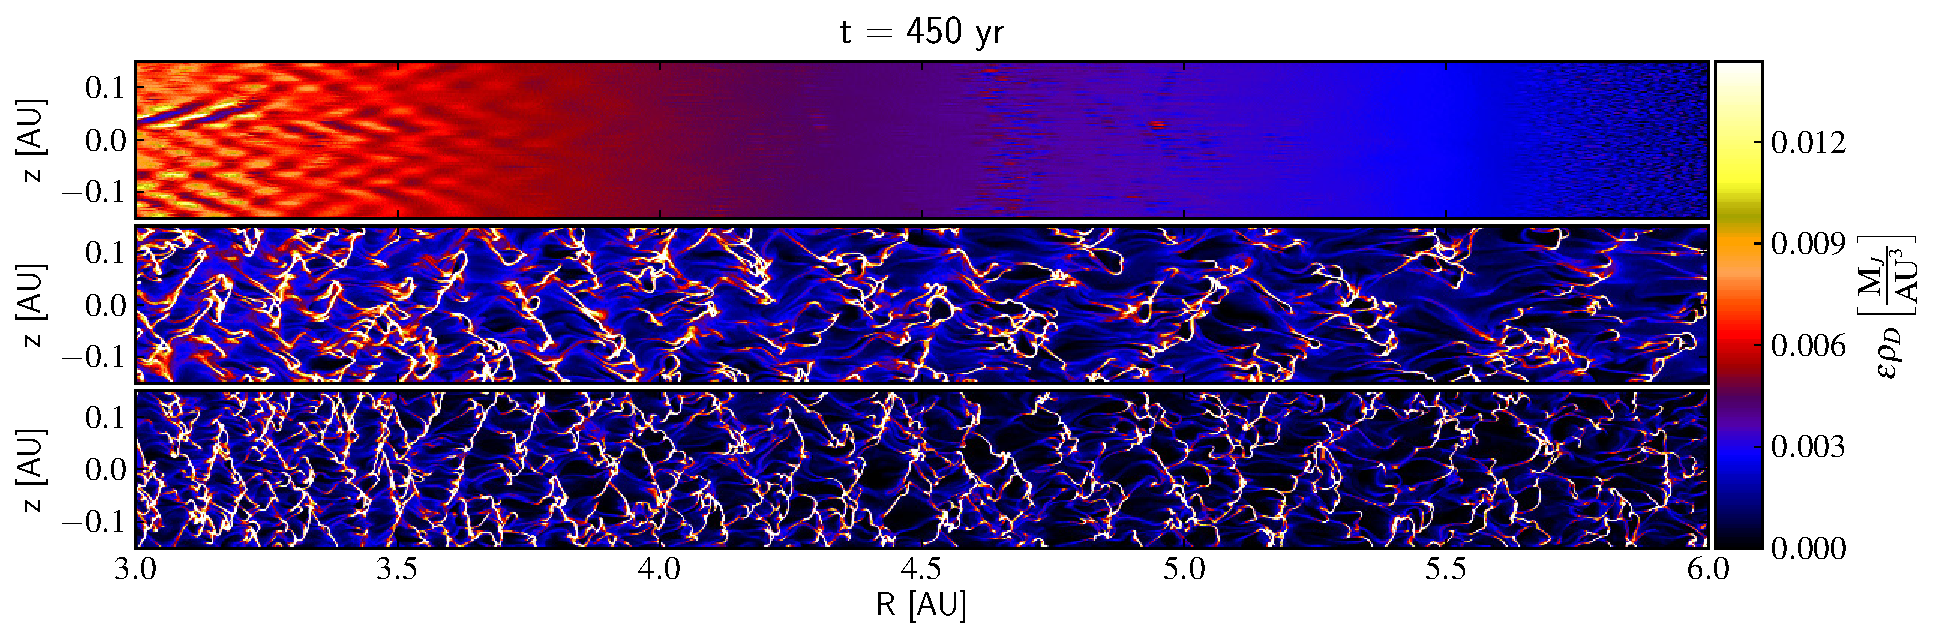
\includegraphics[width=0.99\linewidth]{figures/fig1c}
   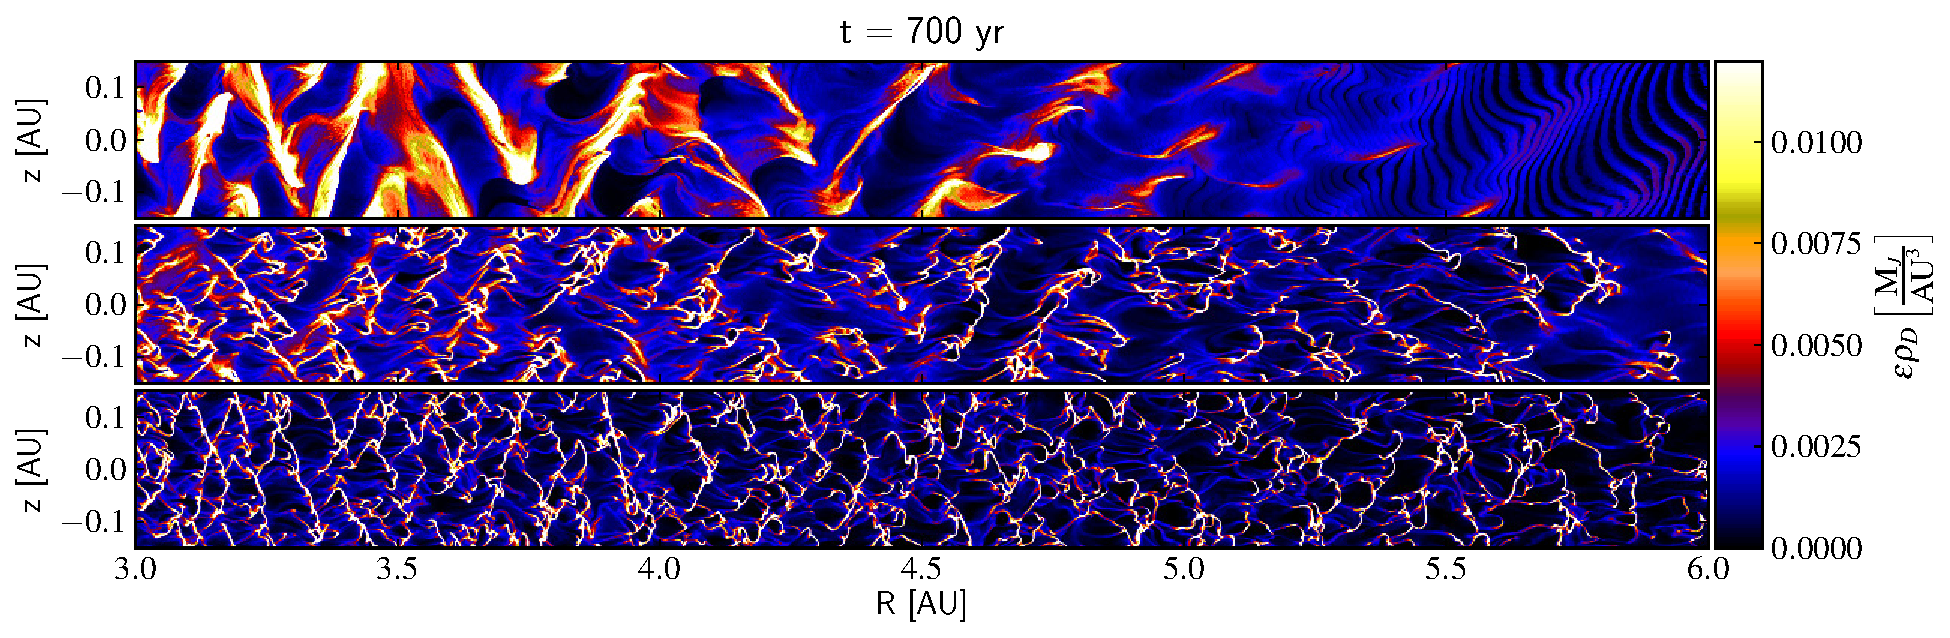
\includegraphics[width=0.99\linewidth]{figures/fig1d}
   \caption{Migawki gęstości pyłu dla symulacji z $50$~cm ziarnami pyłu
      dla czasu $100$, $200$, $450$ oraz $700$~lat odpowiednio dla lewego
      górnego, prawego górnego, dolnego lewego i dolnego prawego panelu.
      Każdy z paneli jest podzielony na trzy części różniące się początkowym 
      $\epsilon = 0.2, 1, 2.0$ odpowiednio dla górnego (BAh), środkowego (BB) i
      dolnego (BC) podpanelu.}
   \label{fig1}
\end{figure*}
%

Niestabilność strumieniowa tworzy najbardziej prominentne struktury pyłu dla
cząstek pyłu o $\tau_s \sim 1$, czyli dla cząstek odsprzęgających się od
dynamiki gazu.
Przy wybranych parametrach symulacji opisanych w rozdziale~\ref{ch2:simpar},
bezwymiarowy parametr ,,stopping time'' jest bliski jedności dla cząstek pyłu o
rozmiarach $50\cm$ (BA, BB, BC). Początkowa liniowa faza ewolucji jest
zdominowana przez wzrost gęstości dla najbardziej niestabilnych modów i prowadzi
do znacznego wzrostu lokalnej gęstości pyłu i uformowania się
charakterystycznych, wydłużonych diagonalnie włókien. W rzeczywistości są to
spłaszczone struktury rozciągające się w kierunku współrzędnej azymutalnej. Po
osiągnięciu nasycenia i przejścia do nieliniowej ewolucji, włókna, na skutek
dużej prędkości w kierunku wertykalnym ulegają fragmentacji i wzajemnie się
przenikają. Jednakże pył dalej poruszą się po charakterystycznych
,,v''--kształtnych trajektoriach, które wytworzyły się podczas liniowej fazy
ewolucji. Migawki z czasowej ewolucji gęstości pyłu zostały przedstawione na
obrazku~\ref{fig1}. Wyraźny jest wpływ początkowego stosunku gęstości pyłu do
gęstości gazu $\epsilon$ na morfologię formujących się obłoków: zarówno ich
typowy rozmiar, jak i kąt nachylenia względem płaszczyzny dysku. Dla $\epsilon =
1$ pył poruszą się i formuje struktury nachylone pod kątem $45^o$, dla
pozostałych przypadków $\epsilon=0.2, 2.0$ kąt nachylenia jest dużo większy,
przez co formujące się struktury są rozciągnięte w kierunku \emph{z}. We
wszystkich wypadkach niestabilność strumieniowa prowadzi do lokalnego wzrostu
gęstości o prawie 2 rzędy wielkości.  Ze względu na swoją gęstość

\subsection{Mocno sprzężony ,,żwir''}
%($a=10\,\textrm{cm}$, $\tau_s\approx 0.24$)
%\label{tight_boulders}}
\begin{figure*}
   \centering
   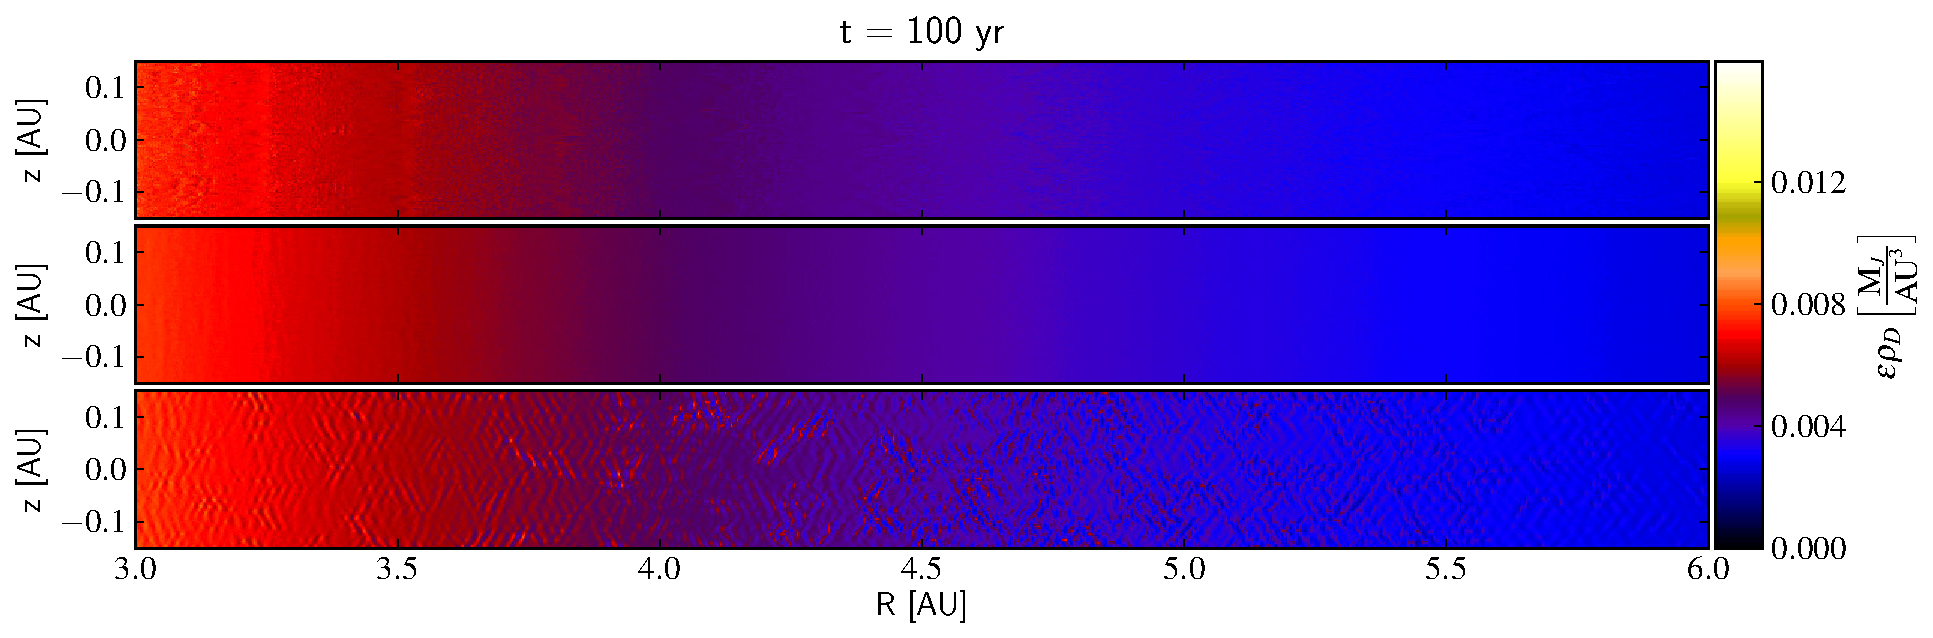
\includegraphics[width=0.99\linewidth]{figures/fig2a}
   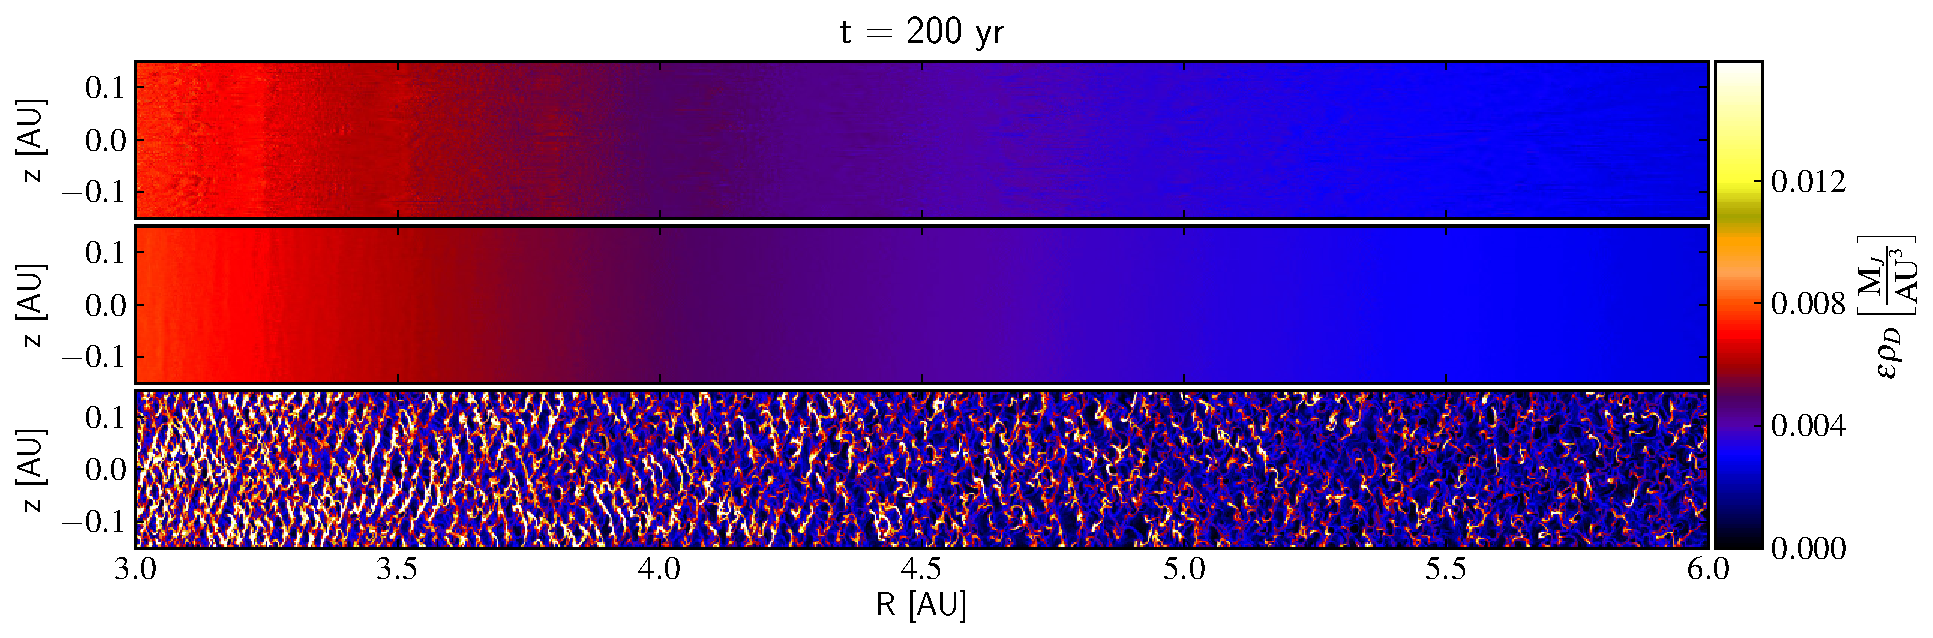
\includegraphics[width=0.99\linewidth]{figures/fig2b}
   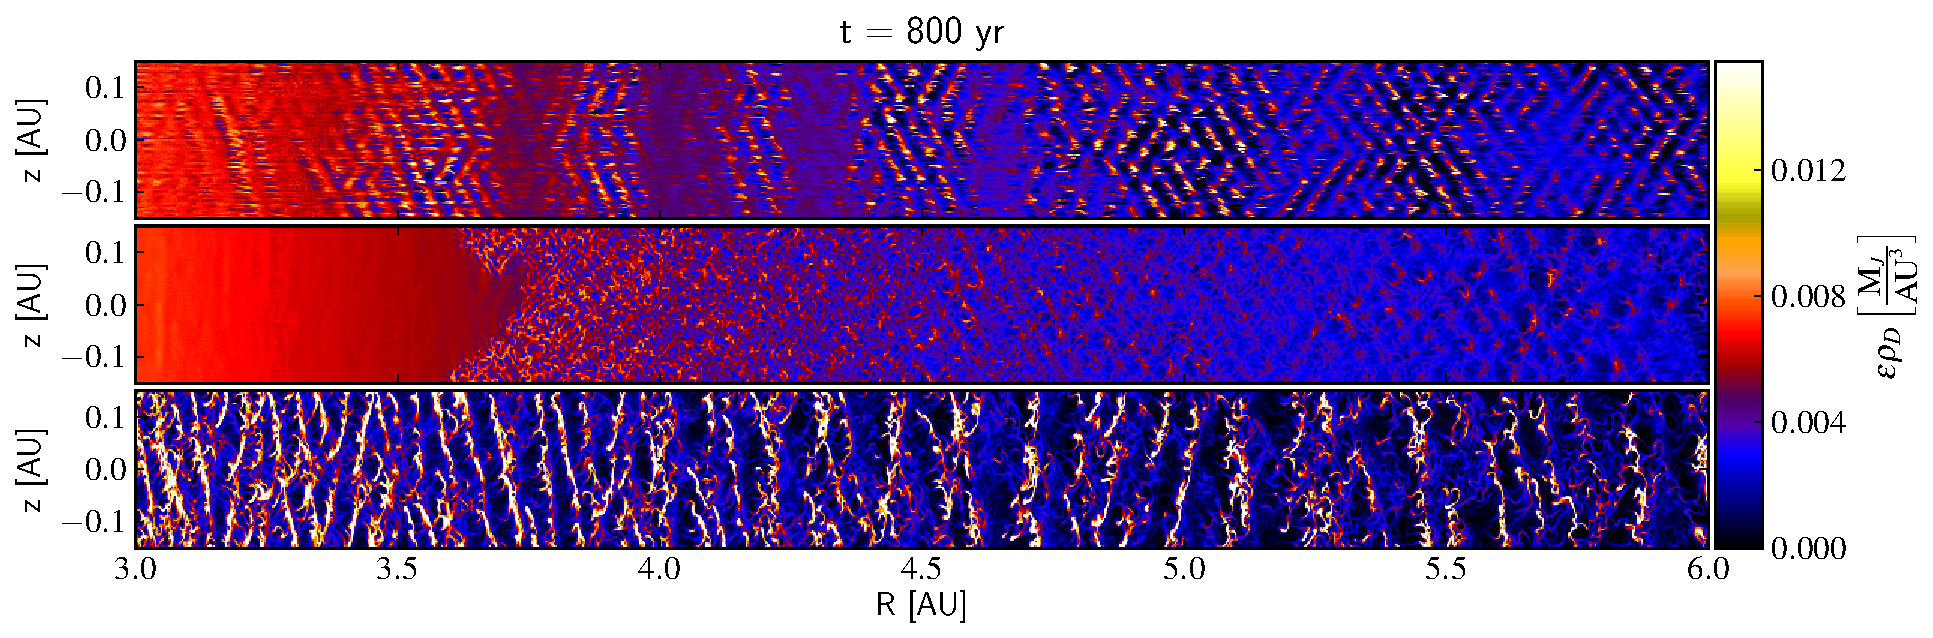
\includegraphics[width=0.99\linewidth]{figures/fig2c}
   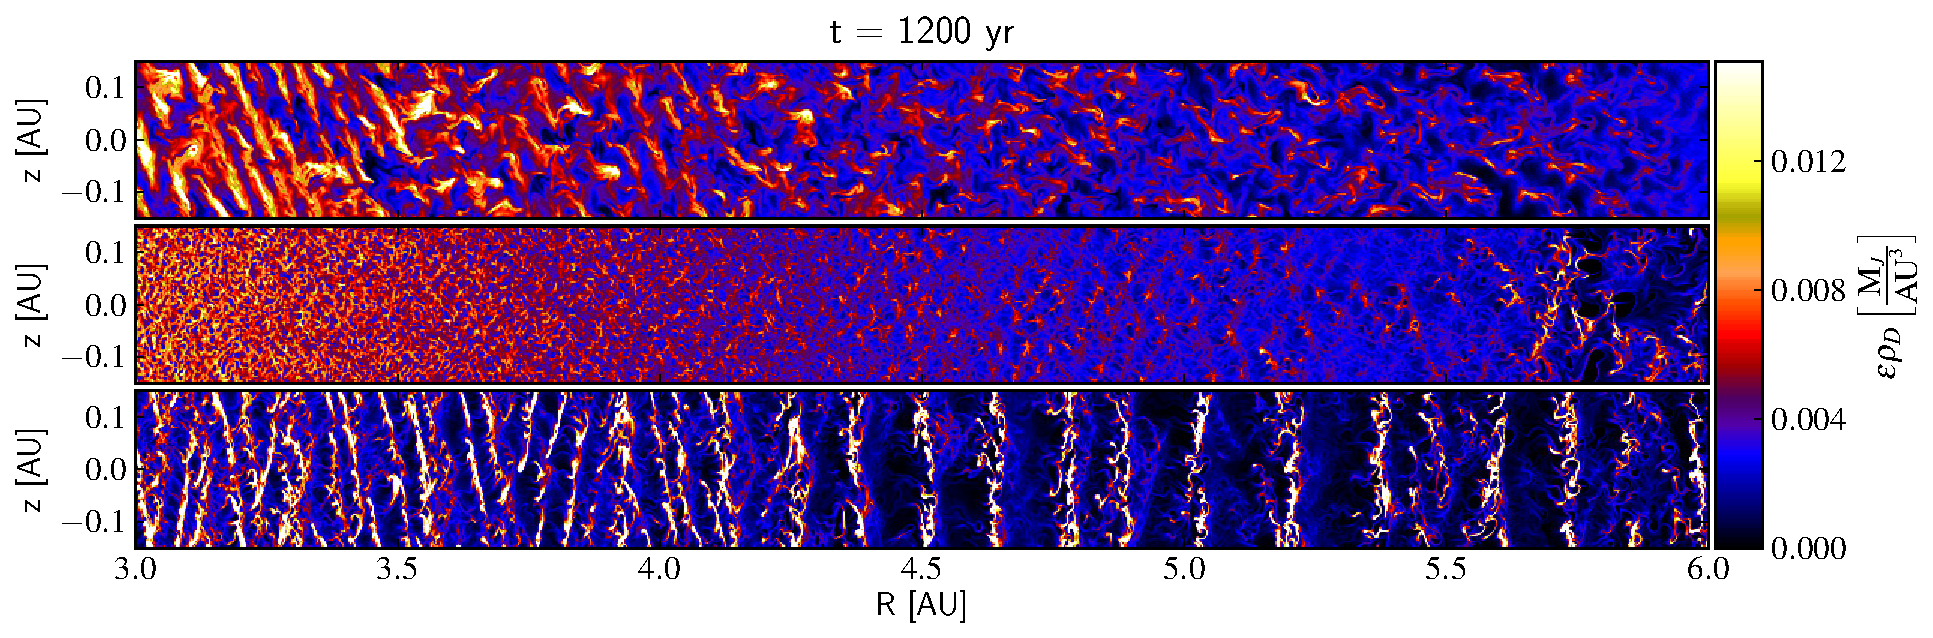
\includegraphics[width=0.99\linewidth]{figures/fig2d}
   \caption{Migawki gęstości pyłu dla symulacji z $10$~cm ziarnami pyłu
      dla czasu $100$, $200$, $800$ oraz $1200$~lat odpowiednio dla lewego
      górnego, prawego górnego, dolnego lewego i dolnego prawego panelu.
      Każdy z paneli jest podzielony na trzy części różniące się początkowym 
      $\epsilon = 0.2, 1, 2.0$ odpowiednio dla górnego (AA), środkowego (AB) i
      dolnego (AC) podpanelu.}
   \label{fig2}
\end{figure*}
Czasowy przebieg symulacji dla silnie sprzężonego pyłu (AA - AC) został
przedstawiony na Rysunku~\ref{fig2}. Ewolucja pyłu dla przypadku $\epsilon =
2.0$ i $10\cm$ ziaren pyłu (AC) nie odbiega znacząco od ewolucji analogicznego
przypadku dla $50\cm$ ziaren pyłu. Liniowa faza niestabilności podczas której
pył zostaje zagęszczony dla najbardziej niestabilnych modów, prowadzi do
wytworzenia się struktur wydłużonych w kierunku wertykalnym. Ze względu na
mniejsze tempo migracji dla sprzężonych cząstek pyłu, zagęszczenia są pochylone
w kierunku radialnym tylko w niewielkim stopniu. Maksymalna gęstość pyłu nie
przekracza dwudziestokrotności wartości początkowej.
\par Przypadek $\epsilon = 0.2$ charakteryzuje się niskim tempem wzrostu. W
początkowej liniowej fazie wzrost lokalnej gęstości pyły prowadzi do uformowania
się charakterystycznej diagonalnej siatki zagęszczeń. Lokalne maksima gęstości
sięgają nawet stukrotnej wielokrotności gęstości początkowej. Jednakże, przejście
do fazy nieliniowej prowadzi do gwałtownego rozmycia skupisk pyłu i osiągnięcia
quasi-stacjonarnego stanu, w którym zagęszczenia podlegają silnej turbulencji,
zaś ich maksymalna amplituda nie przekracza jednego rzędu wielkości względem
stanu początkowego (por. Rysunek~\ref{fig4}).

\par Najciekawszym przypadkiem, zasadniczo odbiegającym od pozostałych, jest
symulacja AB ($\epsilon=1.0,\, a=10\cm$). Początkowo ewolucja przebiega w
identyczny sposób jak dla pozostałych warunków, tzn. pojawia się regularny wzór
w gęstości pyłu odpowiadający najbardziej niestabilnym długościom fal. Jednakże 
po $800$~latach w symulacji AB (mniej więcej dwa razy szybciej w symulacji ABh)
pojawiają się gwałtownie rozszerzające się bąble wypełnione nie wielką ilością
pyłu, które silnie koncentrują pył na swoich brzegach (por. Rysunek~\ref{fig3}). 
Znacząco wzrasta prędkość z którą porusza się pył, po okresie kilkuset lat
silnie turbulentne ruchy propagują się na całą domenę obliczeniową. Ta
specyficzna ewolucja niestabilności strumieniowej jest spowodowana odmiennym
przebiegiem liniowego tempa wzrostu niestabilności (patrz Rysunek~\ref{fig2b)}).
Dla ustalonych parametrów fizycznych AB tempo wzrostu niestabilności $s$ wypada
w punkcie przegięcia funkcji $s(\epsilon)$. Lokalne zwiększenie $\epsilon$ o
tylko $\sim10\%$ przekłada się na dwukrotne zwiększenie tempa wzrostu. Powoduje
to, że drobne zagęszczenia lokalne osiągają nieliniową fazę ewolucji dużo
szybciej niż mniej gęste obszary.  Jest to bezpośrednim powodem obserwowanego
zjawiska, które YJ określili mianem ,,kawitacji''~\footnote{jako analog
gwałtownego pojawiania się bardzo rzadkich bąbli pyłu do nagłego przejścia z
fazy ciekłej do gazowej}.  Turbulencja w pyle prowadzi do wytworzenia się
lokalnych zagęszczeń sięgających rząd wielkości ponad stan początkowy. Jest to
zgodne z wynikami przedstawionymi przez JY07 (patrz Rysunek.~8 w Ich pracy).

\begin{figure} 
\centering
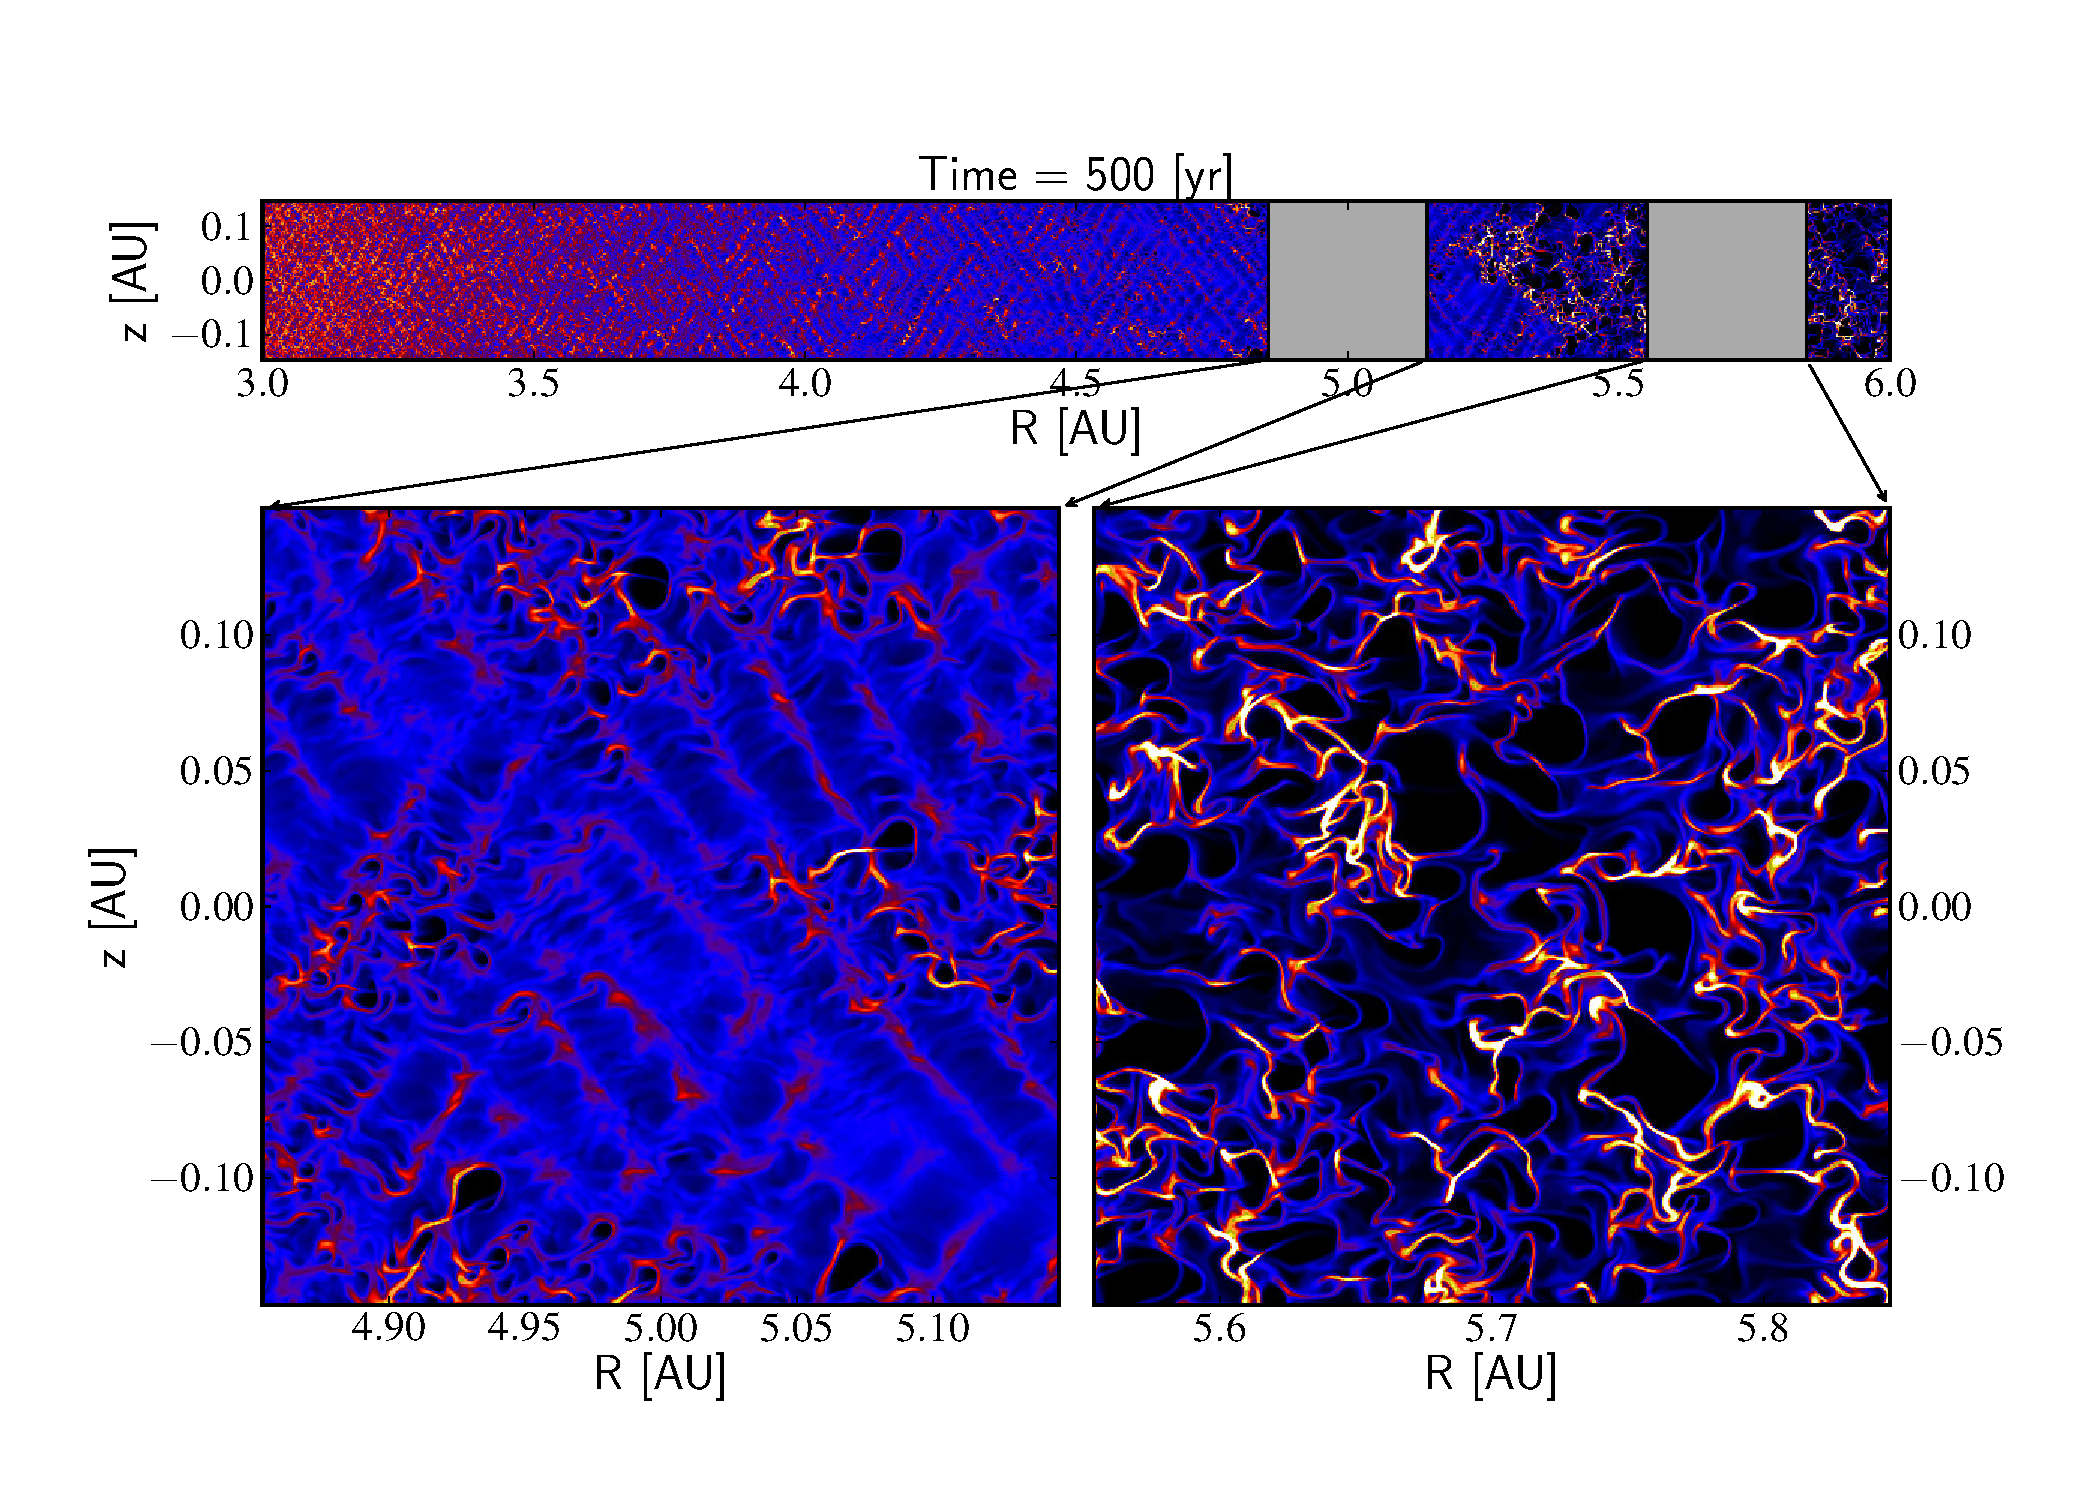
\includegraphics[width=0.98\linewidth]{figures/fig3}
\caption{Migawki gęstości gazu dla symulacji ABh pokazujące dwa ,,zbliżenia''
   obszarów gdzie: występuje pseudo-kawitacja wynikająca z lokalnych zagęszczeń
   wytworzonych w liniowej fazie wzrostu (lewy panel) oraz region całkowicie
   opanowany przez wybuchające bąble pustki i silną turbulencję pyłu (prawy
   panel). Animacja przedstawiająca ewolucję symulacji ABh jest dostępna pod
   adresem \href{http://youtu.be/NoA5-TiQabQ}{http://youtu.be/NoA5-TiQabQ}.}
\label{fig3}
\end{figure}

\begin{figure}
   \centering
   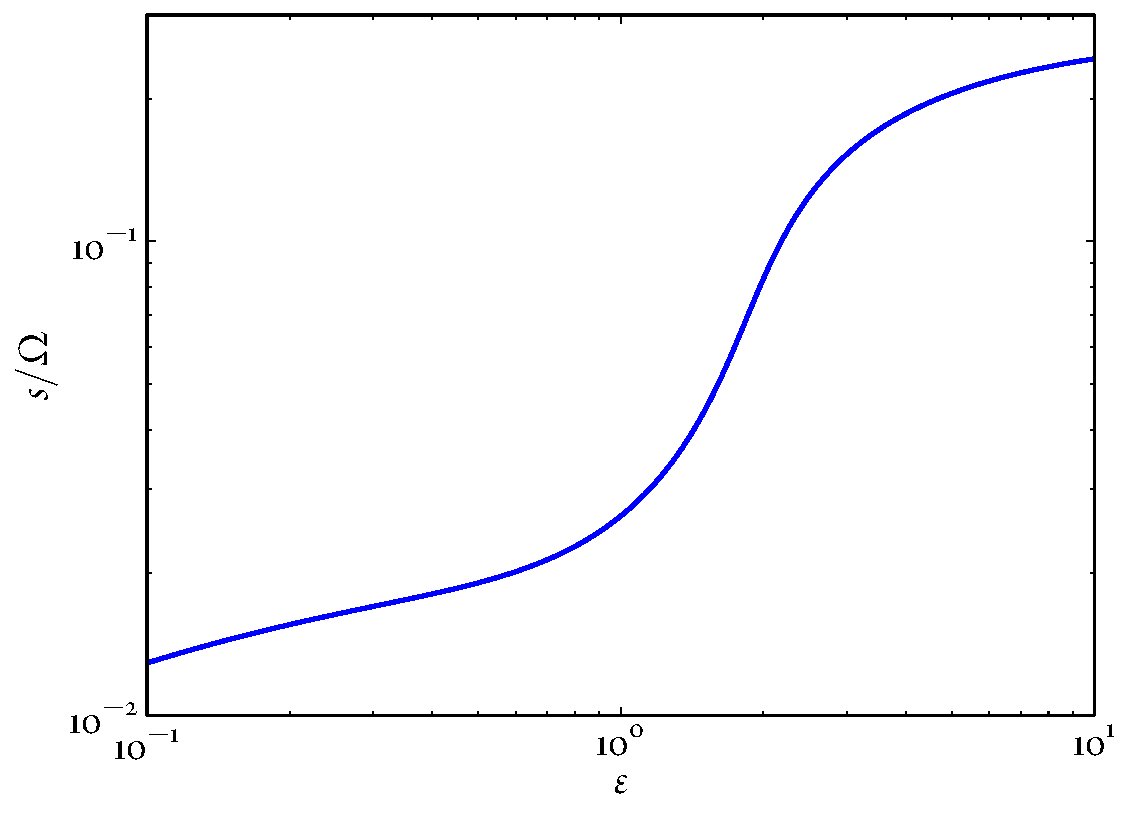
\includegraphics[width=0.5\linewidth]{figures/growthAB}
   \caption{Liniowe tempo wzrostu niestabilności strumieniowej jako funkcja
      stosunku gęstości pyłu do gęstości gazu. Pozostałe parametry niezbędne do
      rozwiązania równania~\mref{eq:disprel} zostały wzięte obszaru znajdującego
   się na lewym panelu Rysunku~\ref{fig2}.}
   %Przełamanie przebiegu funkcji dla
   %   $\epsilon\sim 1$ jest bezpośrednim powodem ,,kawitacji'' obserwowanej w
   %   symulacji AB}
   \label{fig2b}
\end{figure}


\begin{figure}
   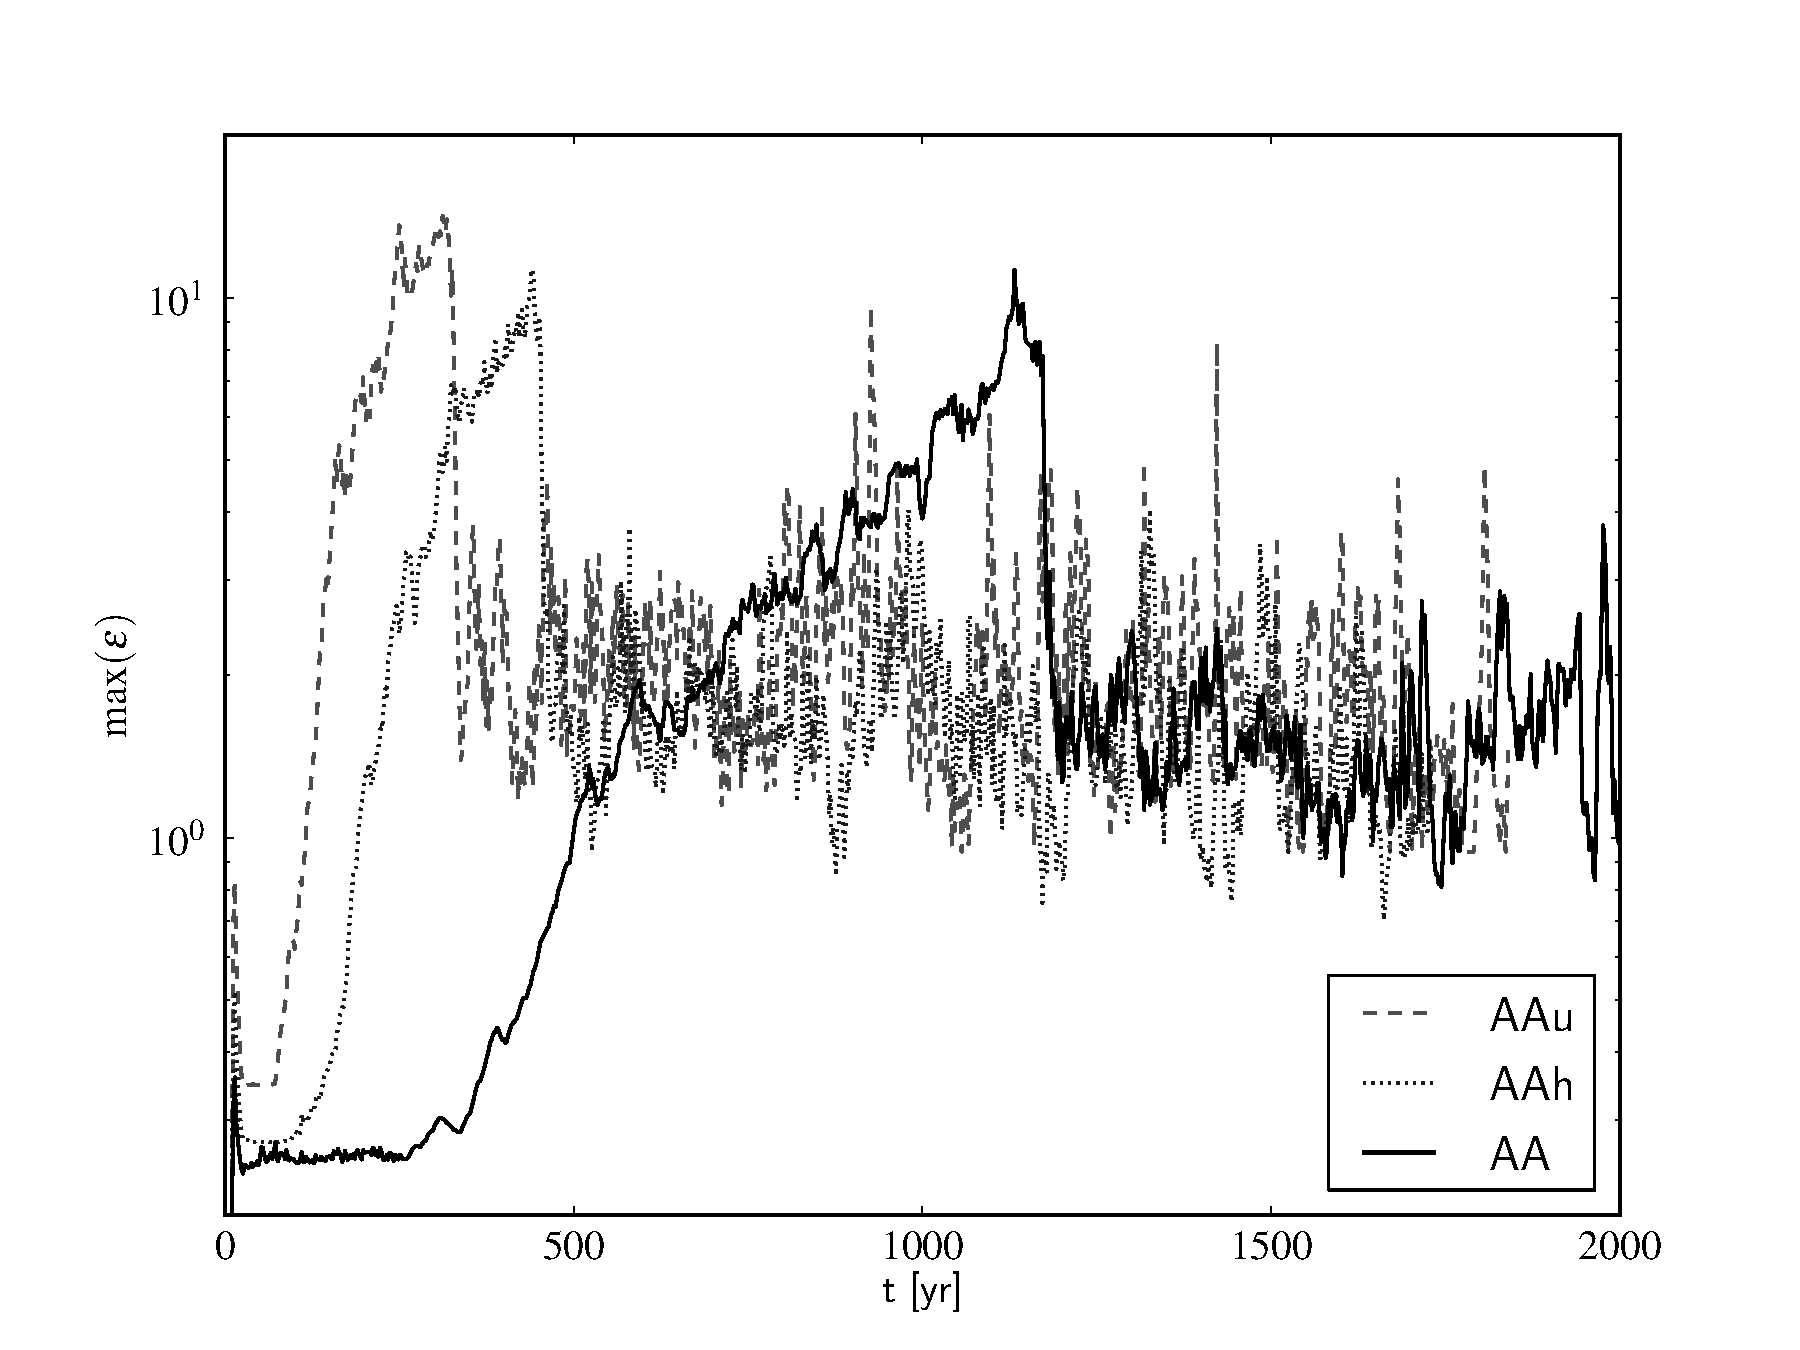
\includegraphics[width=0.98\linewidth]{figures/fig4}
   \caption{
      Maksymalne stosunek gęstości pyłu do gęstości gazu dla trzech symulacji z
      identycznymi, fizycznymi warunkami początkowymi, lecz różną
      rozdzielczością. Ewolucja niestabilności strumieniowej przebiega według
      scenariusza: (1) szybki wzrost podczas liniowej fazy ewolucji, który
      zwiększa lokalnie $\epsilon$ o dwa rzędy wielkości, (2) po
      osiągnięciu krytycznego $\epsilon\approx 10$, zagęszczenia pyłu zostają
      gwałtownie rozmyte, (3) niestabilność osiąga wysycenie, nieliniowa
      ewolucja sprowadza się do oscylacji gęstości pyłu w postaci dużych,
      rozmytych obszarów o maksymalnej gęstości nieprzekraczającej
      dziesięciokrotności wartości początkowej. Zmiana rozdzielczości nie ma
      wpływu na powyższy scenariusz, jedynie wprowadza krótsze i szybciej
   rosnące długości fal skracając etap (1).}

   \label{fig4}
\end{figure}
%

\section{Porównanie wyników z liniową analizą stabilności}
Aby móc porównać obserwowane tempa wzrostu niestabilności strumieniowej z
analizą przedstawioną w rozdziale~\ref{sec:lsa} z domeny obliczeniowej
wyodrębniono małe, kwadratowe ,,łatki'' na wybranych orbitach. Rozmiar wybranych
obszarów $(0.15^2\AU)$ pozwala traktować je w ramach lokalnego przybliżenia
kostki ścinanej, a także umożliwia wyrażenie stałych parametrów występujących w
równaniach \mref{lin1}--\mref{lin4}) poprzez wartości średnie w łatce.
Można zatem przyjąć, że $\bar{\rho}_g = \left<\rho_g\right>$, $\bar{\rho}_d =
\left<\rho_d\right>$ to średnie przestrzenne odpowiednio gęstości gazu i
gęstości pyłu, oraz że ich średni wzajemny stosunek to $\bar{\epsilon} =
\left<\rho_d / \rho_g\right>$. Jako Średnią częstość kątowa $\bar{\Omega}$
przyjęto częstość kątową środka łatki. Bezwymiarowa miara podkeplerowskiej
rotacji jest obliczona zgodnie ze wzorem (patrz YG05 rów.~(16) albo JY07
rów.~(1)).  Wypadku trójwymiarowych symulacji, które dokładnie zostaną opisane
w kolejnych częściach tego rozdziału, ,,łatka'' została wybrana w
płaszczyźnie {\it r-z} dla $\varphi = \varphi_\textrm{max} / 2$.
%
\begin{equation}
   \bar{\eta} = -\frac{c_s^2\left<\partial_R \left<\rho_g\right>_z\right>_R}
      {2\bar{\rho}_g\bar{\Omega}^2 R},
   \label{eq:eta}
\end{equation}
%
W równaniu~\mref{eq:eta} średnia z gęstości gazu jest liczona najpierw w
kierunku wertykalnym, a następnie jest obliczana średnia z radialnej pochodnej 
$\left<\partial_R \rho_g\right>$. Wyrażenie na średni ,,stopping time'' zostało
wyprowadzone z równania~\mref{eq:tauf}
\begin{equation}
   \bar{\tau}_f = \rho_\bullet a / \left(\bar{\rho}_g \sqrt{c_s^2 +
   \left<\left|\mathbf{u} - \mathbf{v}\right|^2\right>} \right).
\end{equation}
%
Dla spójności średnie prędkości gazu i pyłu $\bar{\mathbf{u}},
\bar{\mathbf{w}}$ również są brane jako średnie wartości
$\left<\mathbf{u}\right>, \left<\mathbf{w}\right>$ zamiast obliczania ich przy
pomocy równań~\mref{eq:w0}-\mref{eq:u0} wynikających z założenia dodatkowego
członu w równaniach, niezbędnego w przybliżeniu kostki ścinanej. 
Należy zauważyć, że wartości $\left<\mathbf{u}\right>, \left<\mathbf{w}\right>$,
osiągnięte w sposób naturalny w trakcie trwania symulacji, nie różnią się od
wartości analitycznych o więcej niż $10\%$.
\par Aby określić liniowe tempo wzrostu dla wzbudzanych modów niestabilności
rozkład gęstości i prędkości poszczególnych płynów został przekształcony przy
pomocy transformaty Fouriera, tak aby uzyskać informację o amplitudach
wzbudzanych fal. Analiza przebiegu czasowego zmienności amplitud dla
poszczególnych częstości pozwala wyizolować najbardziej niestabilne mody układy.
Ten etap analizy dla jednej z łatek został przedstawiony na Rysunku~\ref{fig7}.

\begin{figure}
  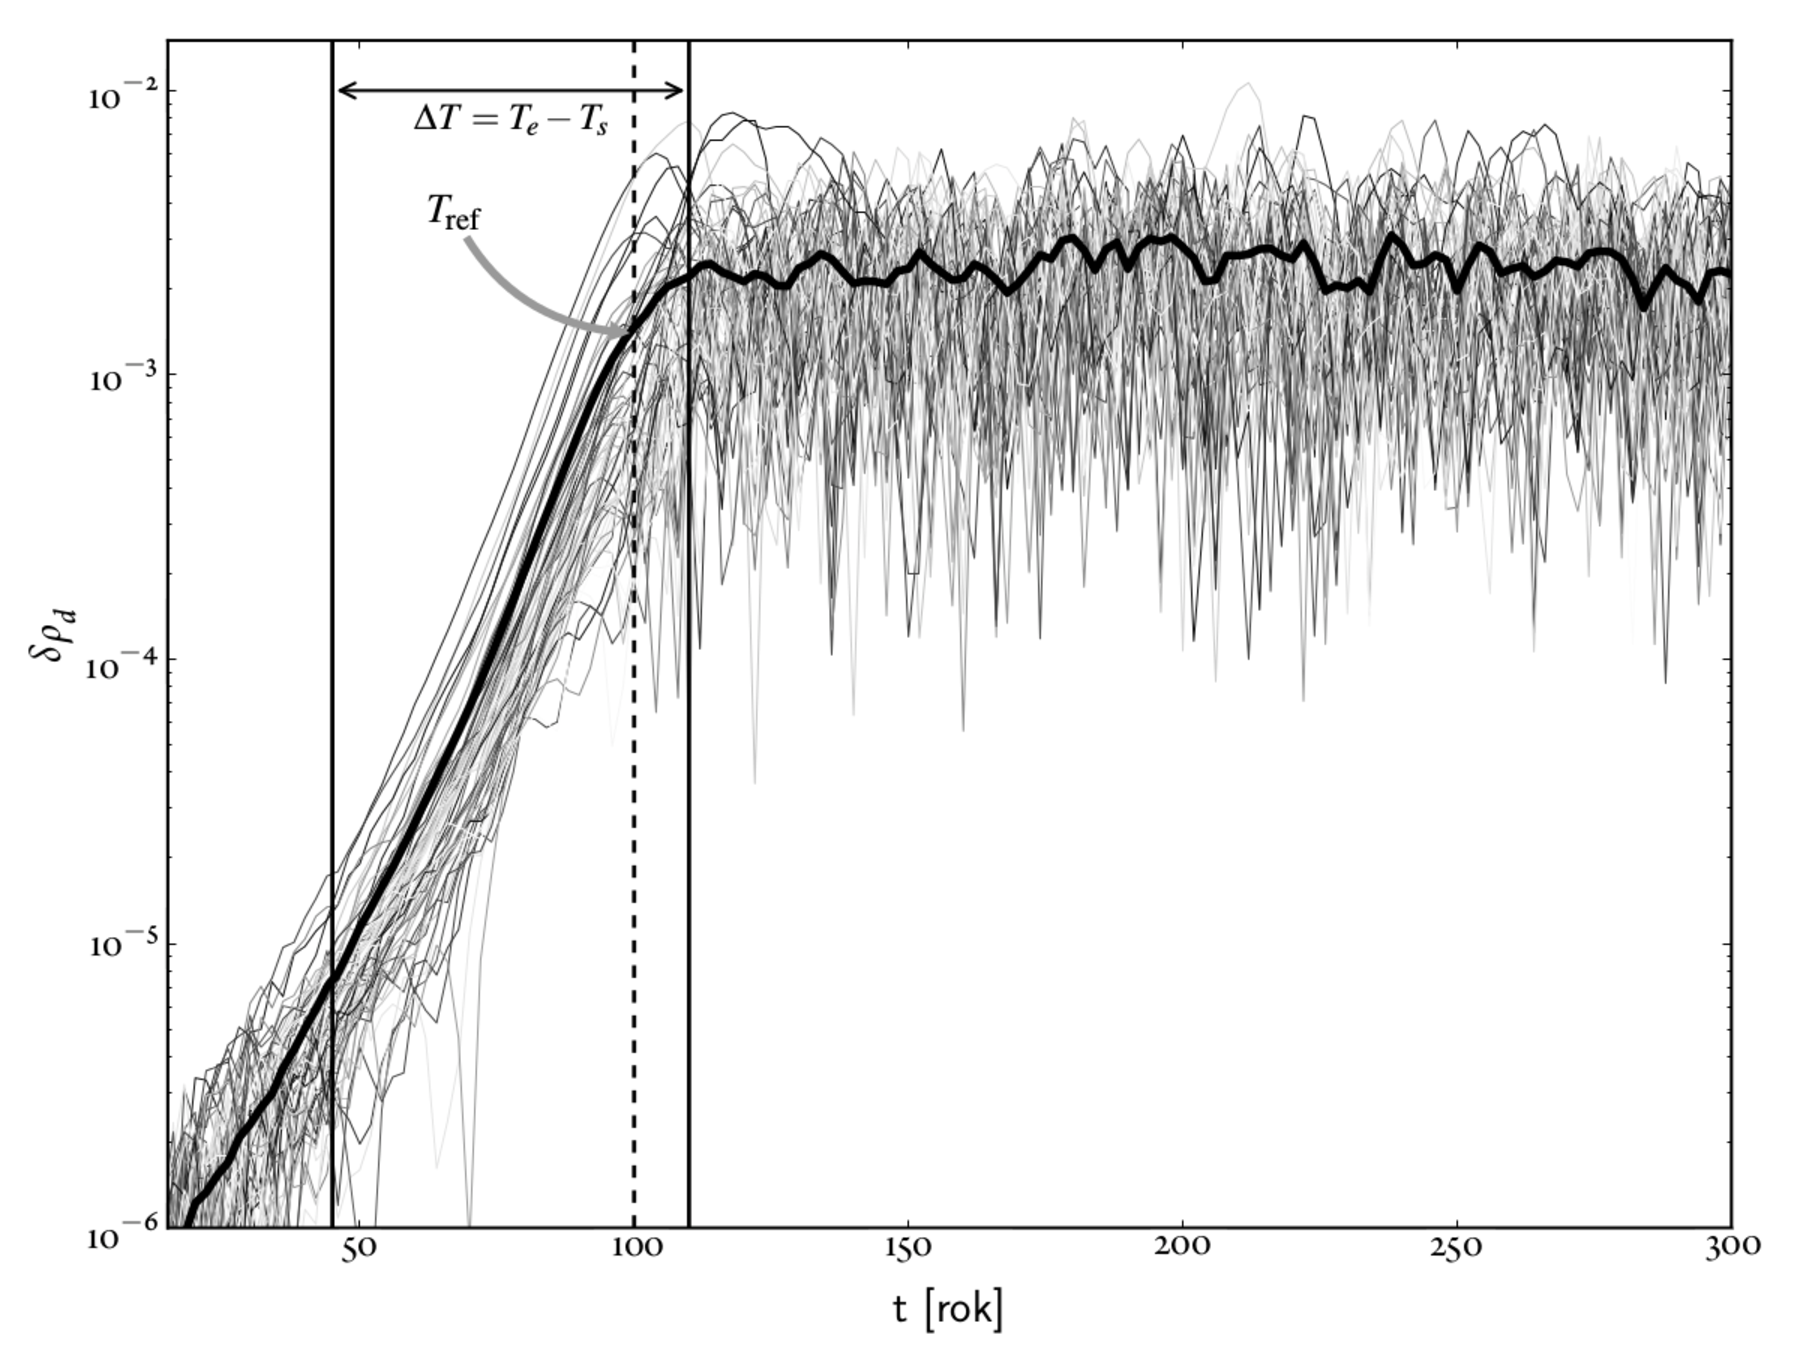
\includegraphics[width=0.98\linewidth]{figures/fig7}

  \caption{Czasowa ewolucja amplitud zaburzenia gęstości pyłu w przestrzeni
     fourierowskiej dla łatki z symulacji BB obejmującej obszar 
     $[2.85,3.15]\times[-0.15,0.15]~\AU^2$. Każda cienka, szara linia
     reprezentuje amplitudę dla wybranej pary liczb falowych $k_x, k_z$.
     $\Delta T = T_e - T_s$ to odcinek czasu dla którego do modów jest
     dopasowywane równanie~\mref{eq:fit}. $T_{\textrm{ref}}$ to punkt
     odniesienia dla którego identyfikowane są dominujące mody na podstawie
     wartości maksymalnej amplitud. Gruba, czarna linia pokazuje uśredniony
     przebieg zmienności dla modów, których amplituda dla $t = T_{\textrm{ref}}$
     jest większa niż $10^{-4}$.} 
   \label{fig7} 
\end{figure}

Dla każdego z badanych obszarów określono czas $T_s$ dla którego część modów
zaczyna wyłaniać się z szumu i rozpoczyna fazę liniowego wzrostu. Na
podobnej zasadzie wyznaczono czas $T_e$, dla którego następuje wysycenie
wzrostu. Następnie do wszystkich modów na przedziale $\Delta T = T_e - T_s$
zostaje dopasowana funkcja
%
\begin{equation}
   f(t) = A\exp\left(-s t\right).
   \label{eq:fit}
\end{equation}
%
Powyższa procedura pozawala na określenie tempa wzrostu w funkcji liczb falowych
$s(k_x, k_z)$ dla wszystkich modów podczas ich liniowego wzrostu. Mody rosnące
najszybciej są określane poprzez znalezienie modów o najwyższej amplitudzie w
wybranym momencie czasu $T_{\textrm{ref}} \lesssim T_e$, tuż przed ich
saturacją. Żadnej z wielkości: $T_s$, $T_e$, $T_{\textrm{ref}}$ nie da się
określić w jednoznaczny sposób. Dla każdej łatki z osobna były one dobierane
arbitralnie na podstawie wizualnej oceny przebiegu dużej ilości modów (patrz
rysunek~\ref{fig7}).  Po określeniu ich tempa wzrostu $s(k_x, k_z)$ jest ono
porównywane z tempem wzrostu $s_0(k_x, k_z)$ wynikającym bezpośrednio z liniowej
analizy dla średnich wielkości płynowych w łatce.

\par Rysunek~\ref{fig8} pokazuje czasową ewolucję amplitud zaburzenia gęstości
pyłu dla 3 najszybciej rosnących modów, wraz z dopasowaną funkcją~\mref{eq:fit}
i tempem wzrostu wynikającym z liniowej analizy dla symulacji BB3d, BB oraz BBh.
Wyraźnie widoczny jest wpływ rozdzielczości na numeryczne tempo wzrostu, a także
zbieżność wyników eksperymentu numerycznego z przewidywaniami teoretycznymi. W
najniższej rozdzielczości tempo wzrostu jest $10\div30\%$ mniejsze niż tempo
analityczne. Ostateczny poziom saturacji dla poszczególnych symulacji znajduje
się na różnym poziomie, ale należy zwrócić uwagę na fakt, że wzrost
rozdzielczości powoduję pojawienie się coraz to krótszych fal, które mogą rosnąć
szybciej i zmieniać obraz całkowity niestabilności strumieniowej.
 
\begin{figure} 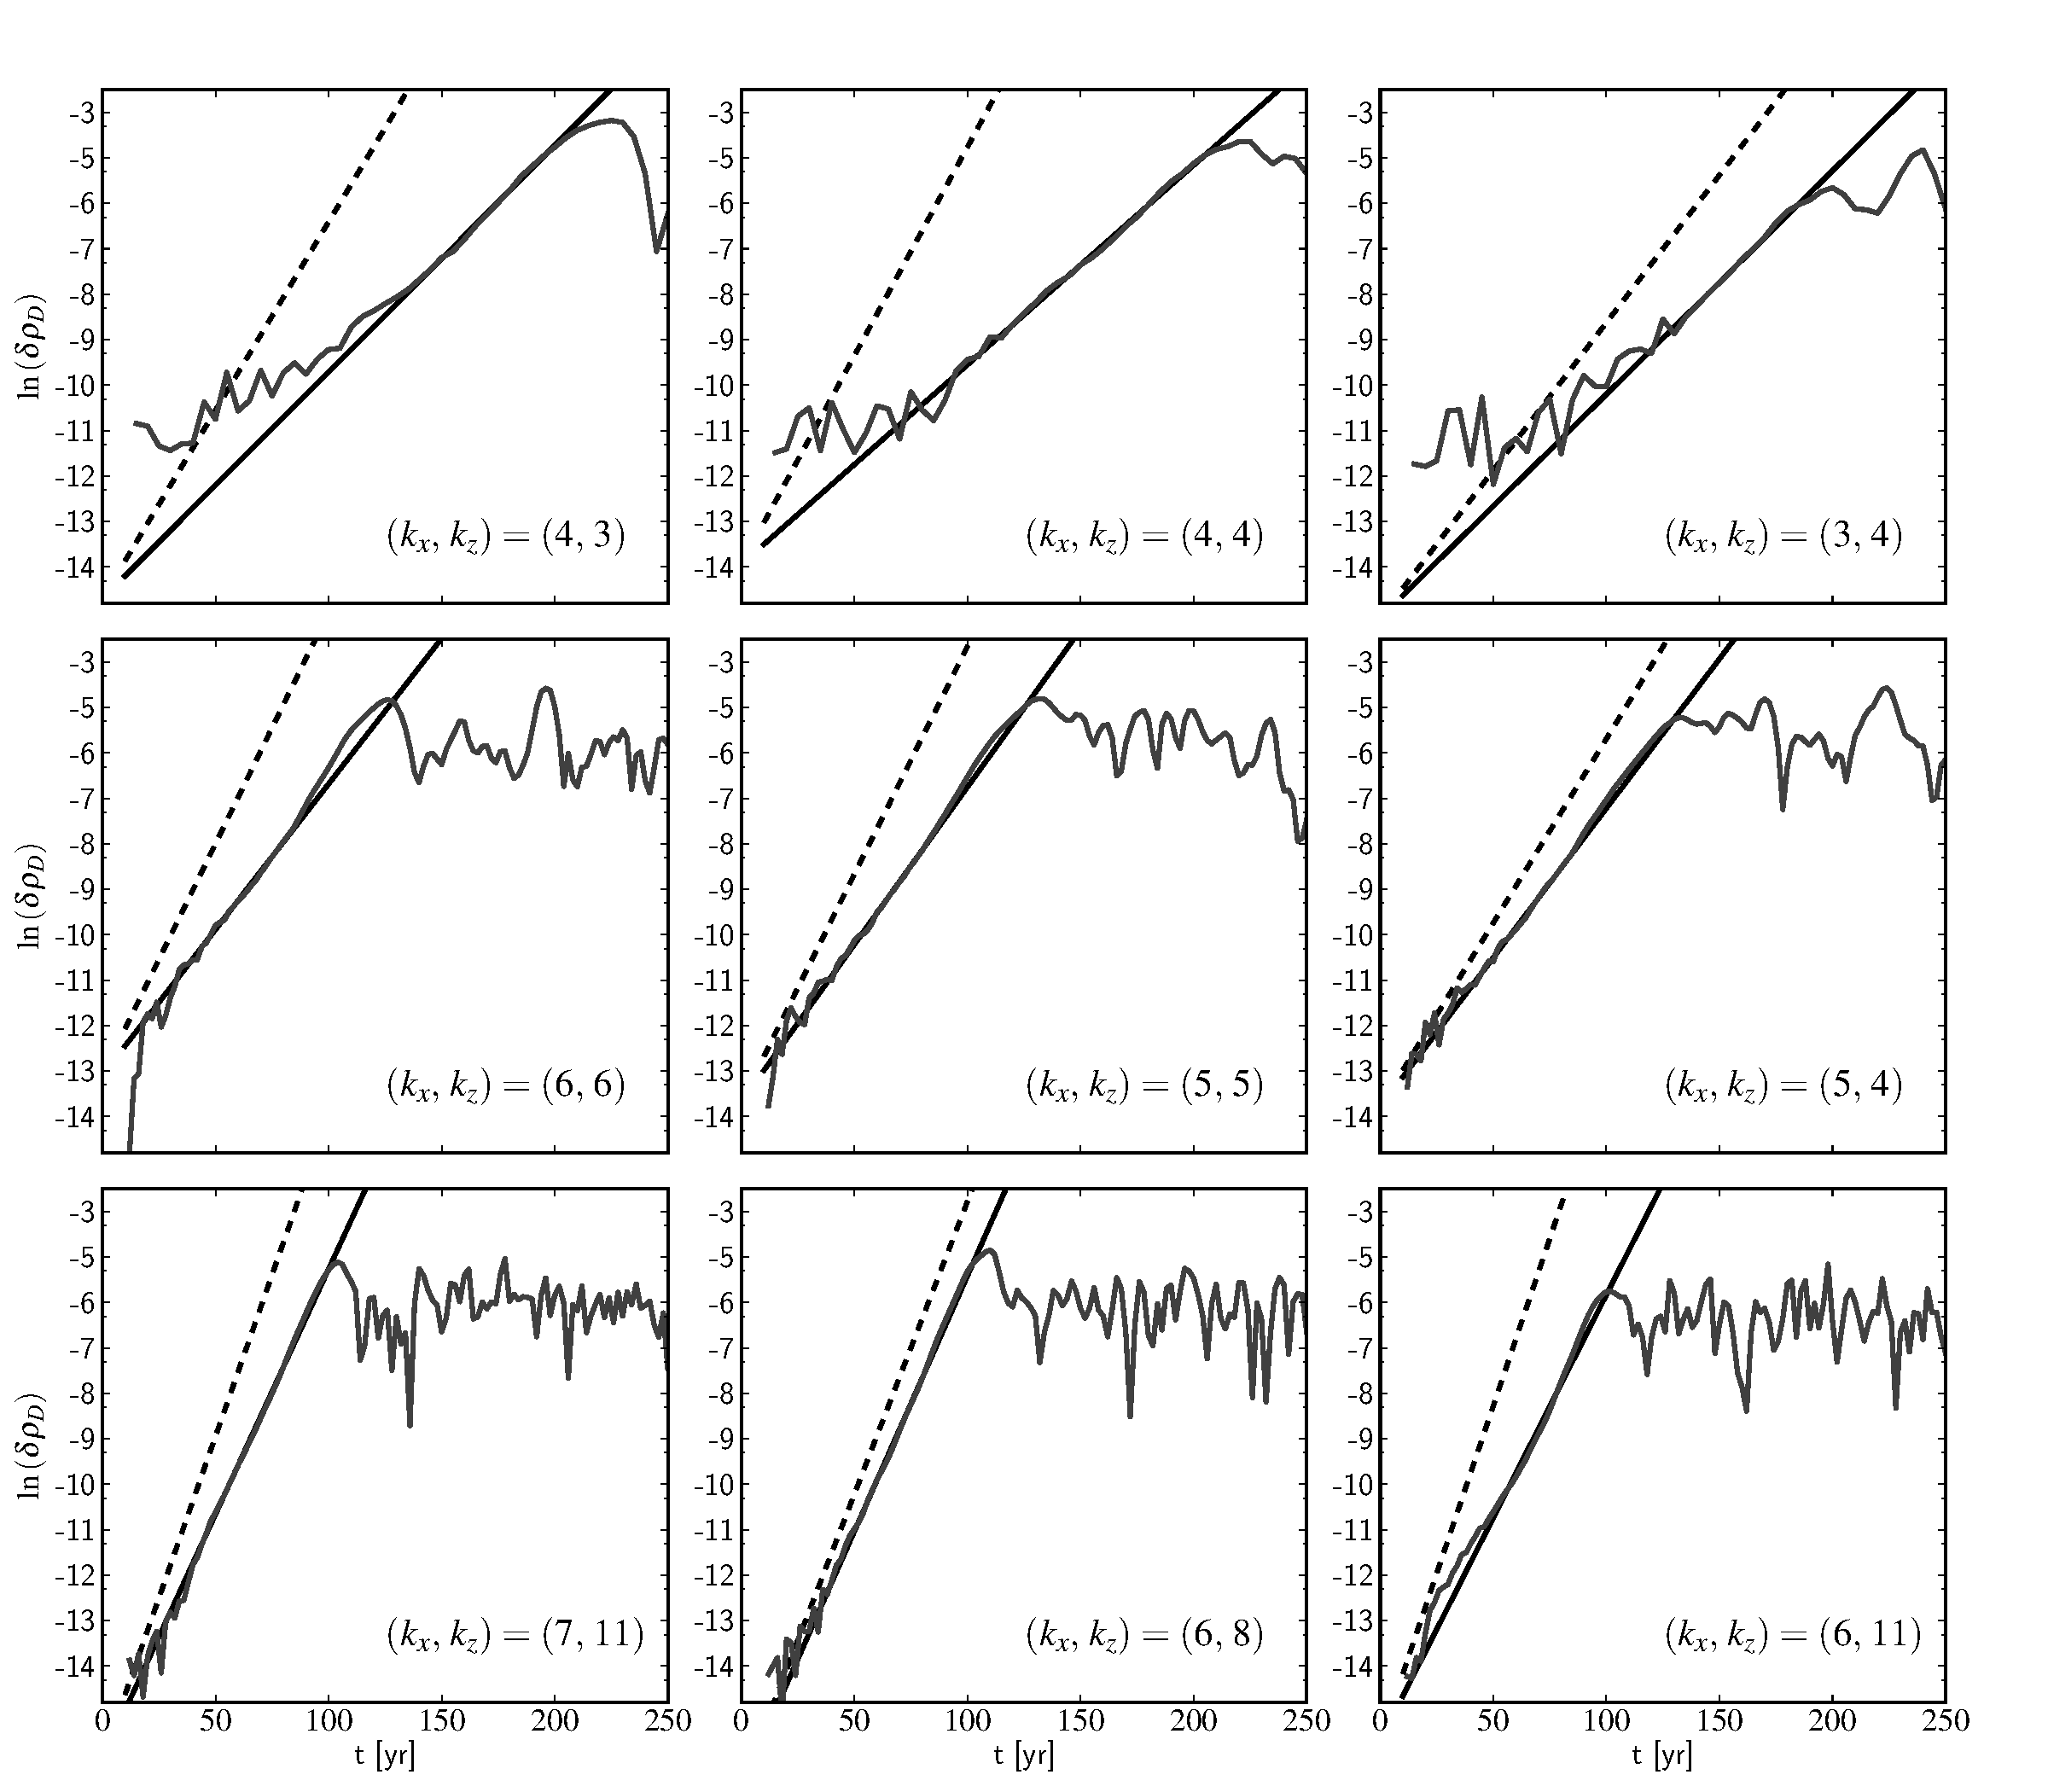
\includegraphics[width=0.98\linewidth]{figures/fig8}
   \caption{Czasowa ewolucja amplitud dominujących modów niestabilności
      strumieniowej mierzona dla zaburzenia gęstości (szara linia) wraz z
      dopasowaniem~\mref{eq:fit} (czarna linia) i przewidywanym tempem wzrostu
      wynikającym z liniowej analizy stabilności (linia przerywana).
      Rozwiązanie równania~\mref{eq:linset} jest określone na podstawie
      parametrów średnich kwadratowej łatki ulokowanej na $R=3\AU$ dla symulacji
BB3d (górny panel), BB (środkowy panel) and BBh (dolny panel).  } \label{fig8}
\end{figure}

\par Kolejnym argumentem potwierdzającym zgodność wyników z liniową analizą
stabilności jest przedstawiony na Rysunku~\ref{fig9} wykres konturowy tempa
wzrostu wynikający z rozwiązania równania~\mref{eq:disprel} w zależności od
liczby falowej. Wyraźnie widać na nim, że najszybciej rosnące mody
niestabilności strumieniowej układają się w charakterystyczny grzbiet w kierunku
rosnących $k_x$ i $k_z$.  Wykres tworzony jest dla stanu średniego w łatce dla
czasu $T_{\textrm{ref}}$.  Następnie 9 dominujących modów wybranych wedle
kryterium opisywanego wcześniej jest zaznaczane przy użyciu punktów. Procedura
jest powtarzana dla symulacji o tych samych parametrach początkowych, ale
różnych rozdzielczościach.  Powyższy schemat działania pozwala potwierdzić, że
liczby falowe dominujących modów wzbudzanych w eksperymencie numerycznym,
układają wzdłuż wspomnianego wcześniej grzbietu. Jedynym czynnikiem
ograniczającym wzrost modów krótkofalowych jest niewystarczająca rozdzielczość
domeny obliczeniowej. Dla serii symulacji BB3d, BB, BBh efektywna rozdzielczość
siatki wyniosła odpowiednio $150^2, 300^2, 600^2$ komórek obliczeniowych.
Dominujące mody symulacji o najniższej rozdzielczości grupują się poniżej
konturu ''$(-1.0)$'', zaś dla najwyższej praktycznie wszystkie mają tempo
wzrostu powyżej $0.1$. Podobne zachowanie jest widoczne dla pozostałych
symulacji dla których przeprowadzono testy zbieżności, tj. AB, ABh (prawy panel
na rysunku~\ref{fig9}). Przypuszczalnym powodem obecności wyraźnego obcięcia dla
krótki długości fali w przeprowadzonych symulacjach jest wewnętrzną, numeryczna
dyfuzyjność metody RTVD użytej w PIERNIKu. Z przeprowadzonych analiz wynika, że
używane algorytmy numeryczne potrzebują przynajmniej 32 komórek obliczeniowych
na długość fali niestabilnego modu, aby poprawnie oddać jego tempo wzrostu.
Należy przy tym zauważyć, że krótsze mody zawierające się w mniejszej liczbie
komórek nadal pozostają niestabilne, aczkolwiek mogą wykazywać mniejsze tempo
wzrostu niż to wynikające z liniowej analizy stabilności.

\begin{figure*}
  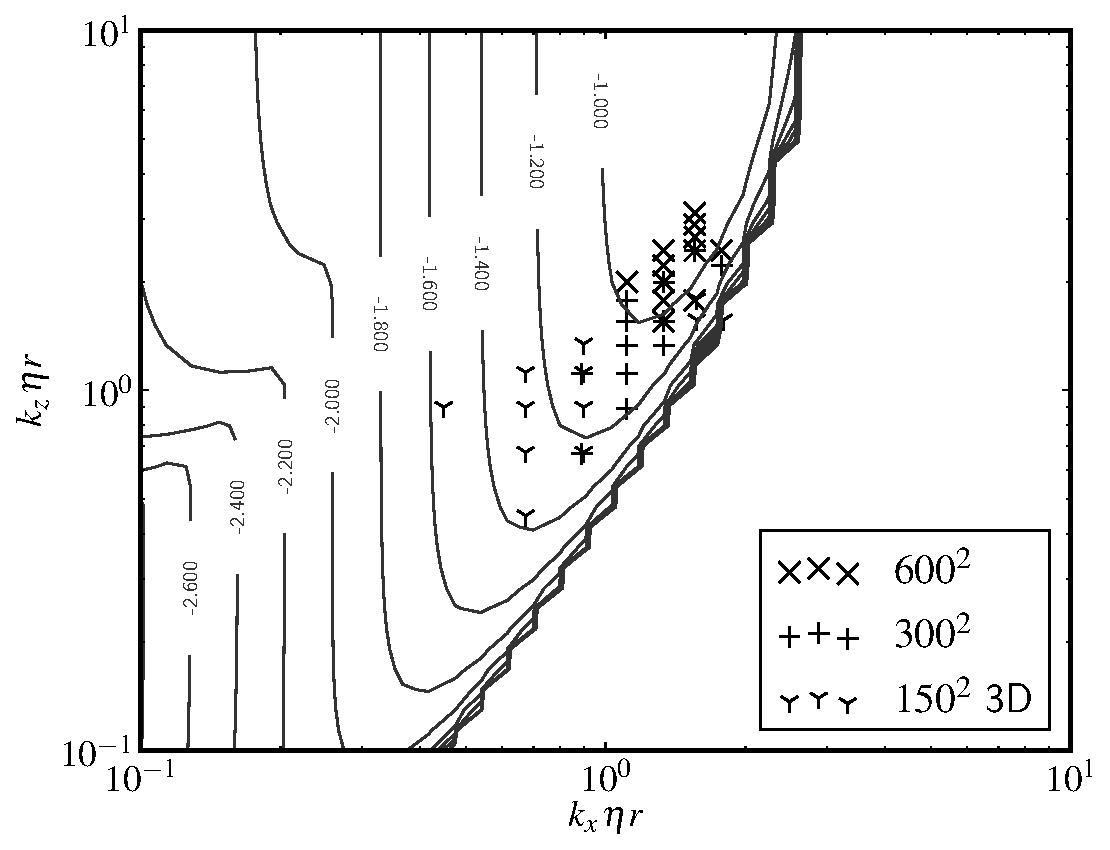
\includegraphics[width=0.48\linewidth]{figures/fig9a}
  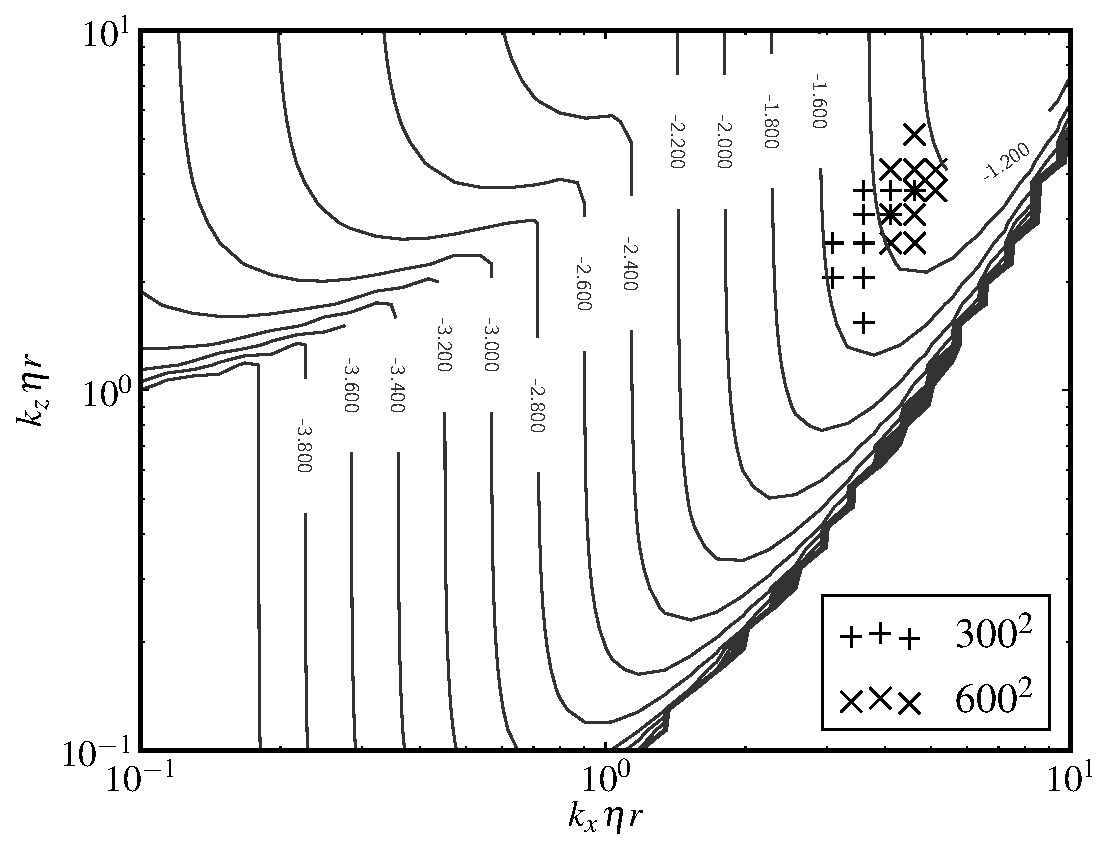
\includegraphics[width=0.48\linewidth]{figures/fig9b}
  \caption{Dziewięć najszybciej rosnących modów o liczbach falowych $(k_x, k_z)$
     wyodrębnionych z symulacji o tych samych fizycznych warunkach początkowych,
     lecz różnej rozdzielczości siatki obliczeniowej. (lewy panel: BB3d, BB,
     BBh, prawy: AB, ABh). Kontury wyznaczają tempo wzrostu $\log_{10}( s_0(k_x,
  k_z))$ wynikające z rozwiązania równania~ \mref{eq:disprel} dla średniego
  stanu wybranych łatek w momencie czasu  $T = T_{\textrm{ref}}$ (dla porównania
  por. Rysunek.~2 z pracy~\cite{YG05})}
   \label{fig9}
\end{figure*}
 
% \subsection{Convergence}
\par Jako że niestabilność strumieniowa w ogólności ,,preferuje'' krótsze
długości fali, zwiększenia rozdzielczości zawsze prowadzi do wytworzenia
to zagęszczeń o coraz mniejszych rozmiarach w krótszym czasie~(por.
Rysunek~\ref{fig10}).  Jednakże przeprowadzone symulacje odtwarzają w dobrym
stopniu przewidywania liniowej analizy stabilności, a także są w stanie oddać
wszystkie efekty jakościowe, np. ,,kawitację'' (por. Rysunek~\ref{fig3}) czy
gwałtowne rozmycie niestabilności w przypadku $\epsilon=0.2$ i $a=10\cm$, bez
względu na rozmiar najmniejszej komórki obliczeniowej.

\begin{figure}
   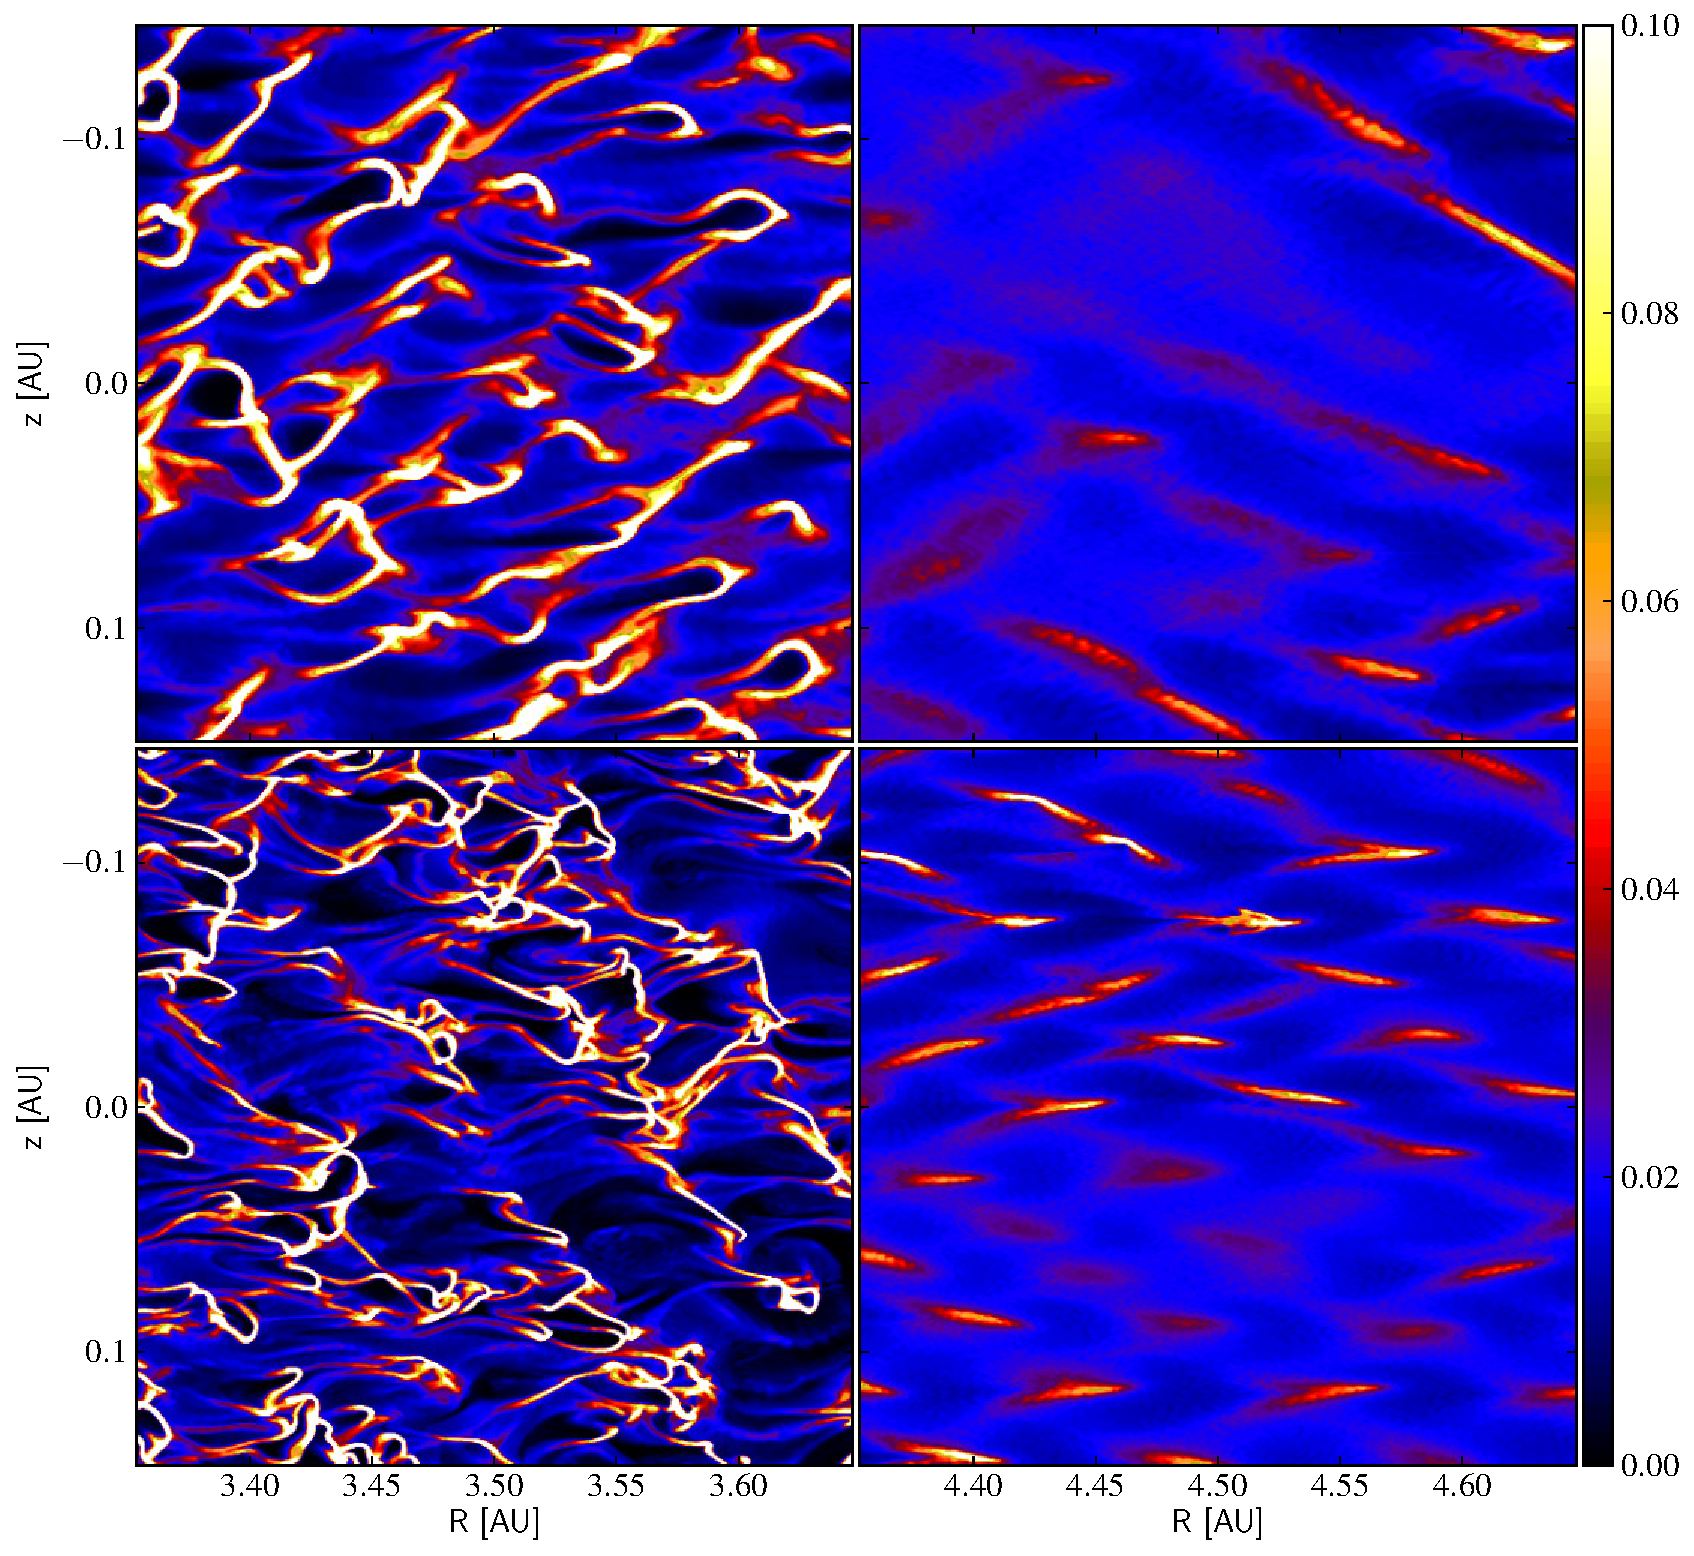
\includegraphics[width=0.98\linewidth]{figures/fig10}
   \caption{Migawki gęstości pyłu dla $t = 160\yr$ dla łatek pochodzących z
      orbit $R=3.5$ i $4.5\AU$ wyodrębnione z symulacji o tych samych warunkach
      początkowych lecz różnej rozdzielczości siatki obliczeniowej. Górny panel
      symulacja BB, zaś dolny symulacja BBh. Ze względu na właściwości
      dyfuzji numerycznej, wyższa rozdzielczość promuje krótsze długości
      fali}
   \label{fig10} 
\end{figure}

\section{Symulacje trójwymiarowe}
W ramach poniższej pracy przeprowadzono 2 rodzaje symulacji pełnego,
trójwymiarowego modelu dysku: z uwzględnieniem efektów samograwitacji płynów
(BD3dS) oraz bez jej udziału (BB3d, BD3d). Symulacja BB3d została przeprowadzana
w celu ścisłego porównania wyników z analogicznymi symulacjami dwuwymiarowymi.
Podobnie jak w przypadku zredukowanym, ewolucja niestabilności strumieniowej
przebiega głównie w płaszczyźnie \textit{r-z}. Początkowo w gęstości pyłu
wyłania się przedstawiony już wcześniej ukośny wzór, będący wynikiem działania
najbardziej niestabilnych modów. Wydłużone zagęszczenia pyłu formują warstwy
rozciągające się na cały dysk w kierunku azymutalnym. Odstępstwa od osiowej
symetrii są zauważalne, lecz praktycznie nie wpływają na zachowanie się
niestabilności (por. Rysunek~\ref{fig:slicenosg}. Podobnie jak w analogicznych
symulacjach 2D, saturacja niestabilności następuje po lokalnym wzroście gęstości
pyłu o $1\div1.5$ rzędu wielkości.
%
\begin{figure}
   \centering
   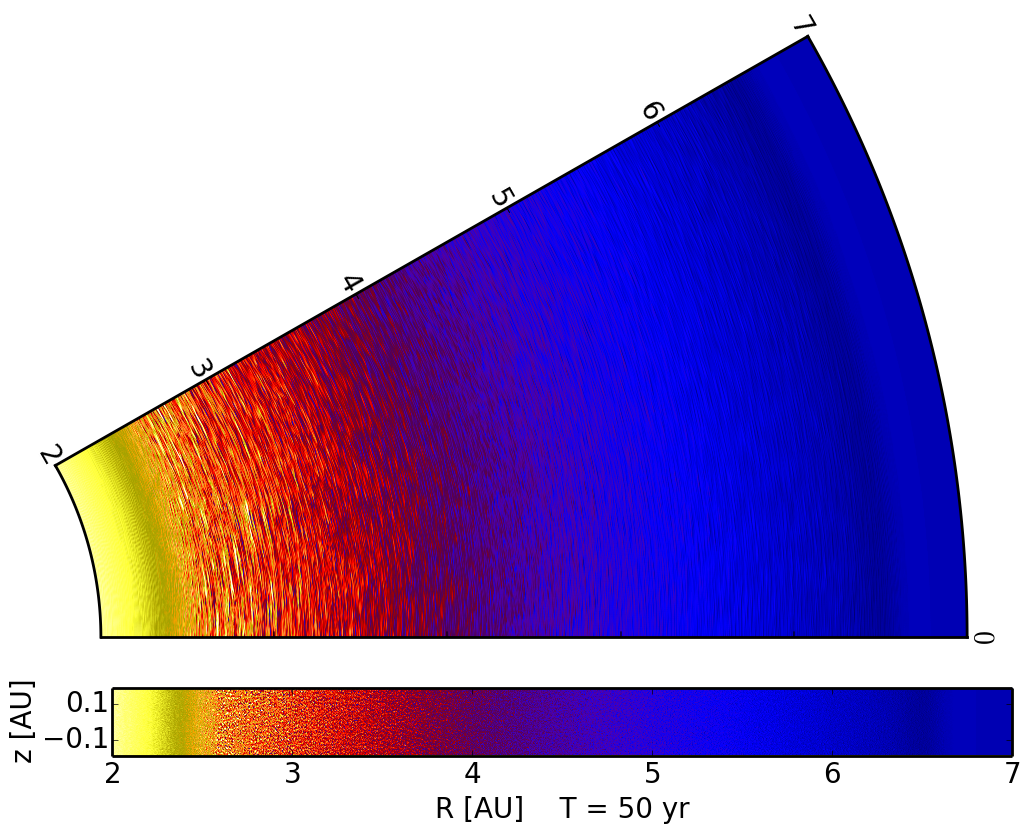
\includegraphics[width=0.44\linewidth]{figures/slice_nosg_01}
   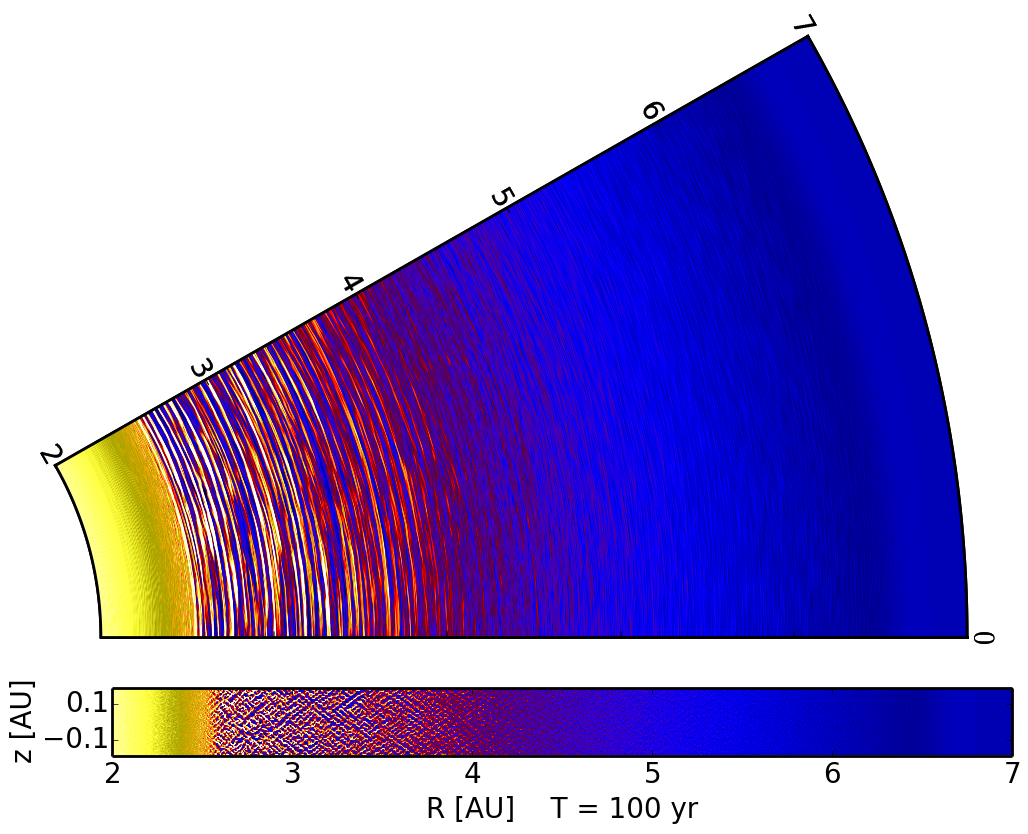
\includegraphics[width=0.44\linewidth]{figures/slice_nosg_02} \\
   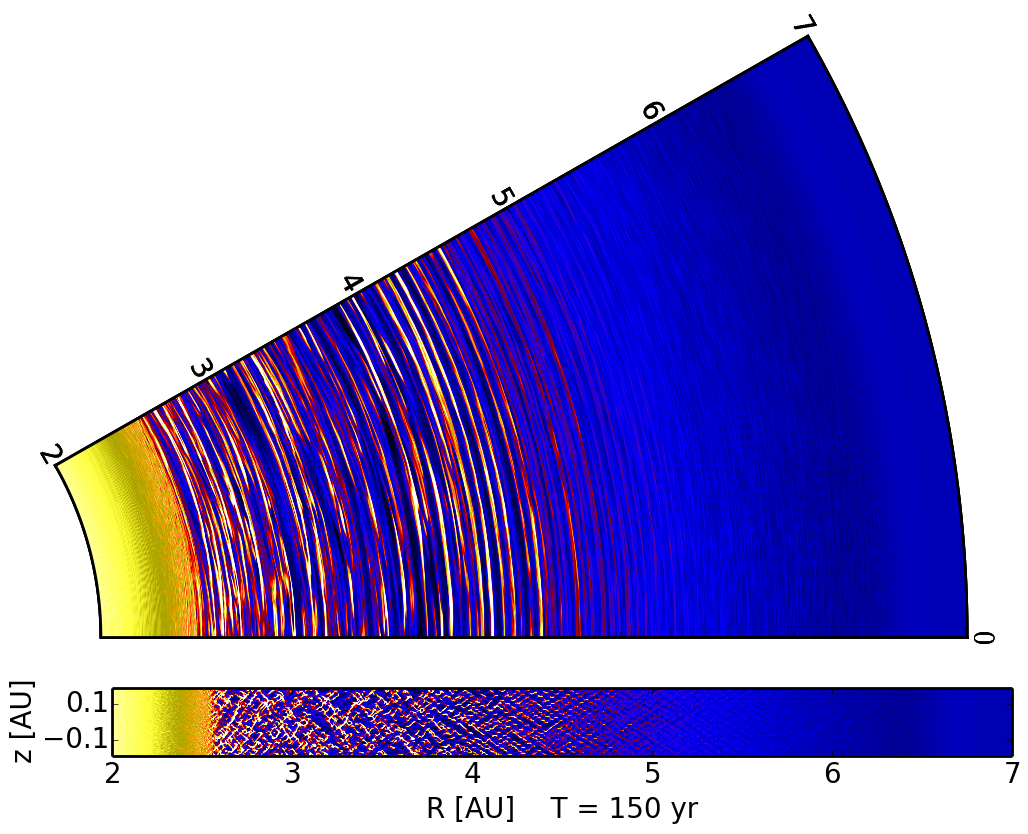
\includegraphics[width=0.44\linewidth]{figures/slice_nosg_03}
   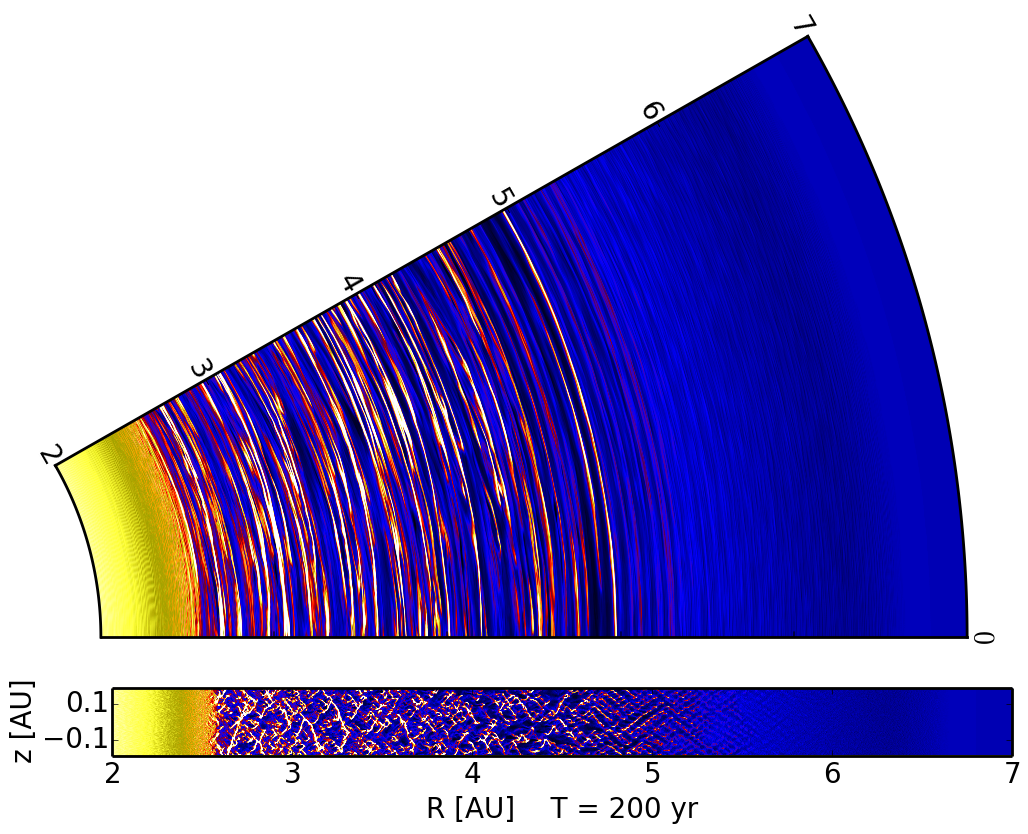
\includegraphics[width=0.44\linewidth]{figures/slice_nosg_04} \\
   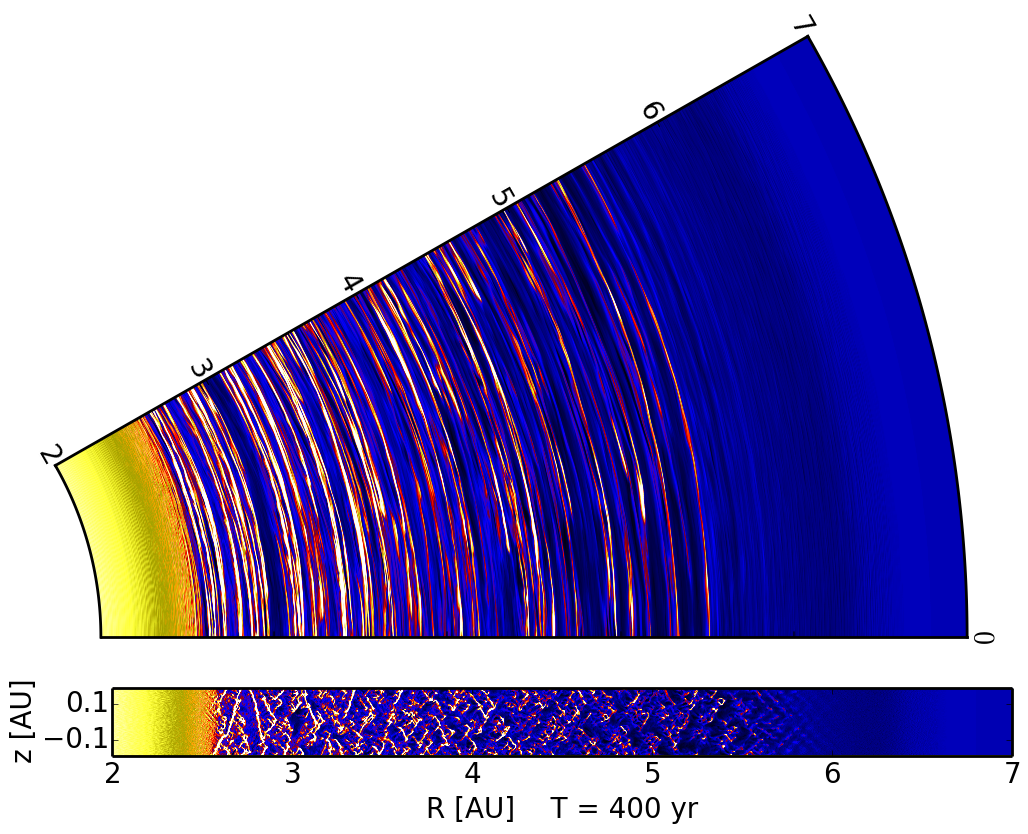
\includegraphics[width=0.44\linewidth]{figures/slice_nosg_05}
   \caption{
      Migawki z symulacji BD3d obrazujące gęstość pyłu w cięciach w
      płaszczyznach $R -\varphi$ oraz $R - z$ przechodzących przez środek 
   domeny obliczeniowej, dla czasów $T= 50, 100, 150, 200, 400$}
   \label{fig:slicenosg}
\end{figure}
%
\par Obraz niestabilności strumieniowej diametralnie się zmienia po
uwzględnieniu samograwitacji pyłu. Początkowo ewolucja przebiega wzdłuż tego
samego scenariusza, dominujące mody niestabilności strumieniowej formują
charakterystyczny wzór--kratkę (Rysunek~\ref{fig:slicesg}). Tempo tworzenia się
zagęszczeń w tej fazie $(50 - 100\yr)$ jest takie samo jak w przypadku bez
samograwitacji~(Rysunek~\ref{fig:modes3d}). Ponadto dominujące mody lokują się
na mapie stabilności w obszarze o największym tempie wzrostu wynikającyc z
liniowej analizy (Rysunek~\ref{fig:map3d}).  Pierwsza zauważalną różnicą jest
przekroczenie przez pył gęstości na której wcześniej niestabilność strumieniowa
się wysycała (por. środkowy panel na Rysunku~\ref{fig:hists}). Jest to prostą
konsekwencją faktu, że każde formujące się zagęszczenie jest dodatkowo
wspomagane działającą do wewnątrz siłą samograwitacyjną. Po $150$~latach dysk
pyłowy staje się dużo bardziej pofragmentowany w kierunku azymutalnym.
Odstępstwo od osiowej symetrii jest wyraźnie zauważalne. Warstwy gęstego pyłu na
skutek wzajemnego oddziaływania grawitacyjnego (jak i własnego ciężaru)
zaczynają się deformować coraz silniej zmieniając swoją strukturę w kierunku
azymutalnym. W ciągu kolejnych $50$~latach samograwitacja ,,ściska'' praktycznie
cały pył do jednej płaskiej warstwy w płaszczyźnie $R - \varphi$ w formie
długich pofalowanych włókien (Rysunek~\ref{fig:projs}). W toku dalszej ewolucji
włókna fragmentują na mniejsze związane grawitacyjnie obiekty -- planetezymale,
które podlegają dalszym oddziaływaniom dynamicznym. 

%
\begin{figure}
   \centering
   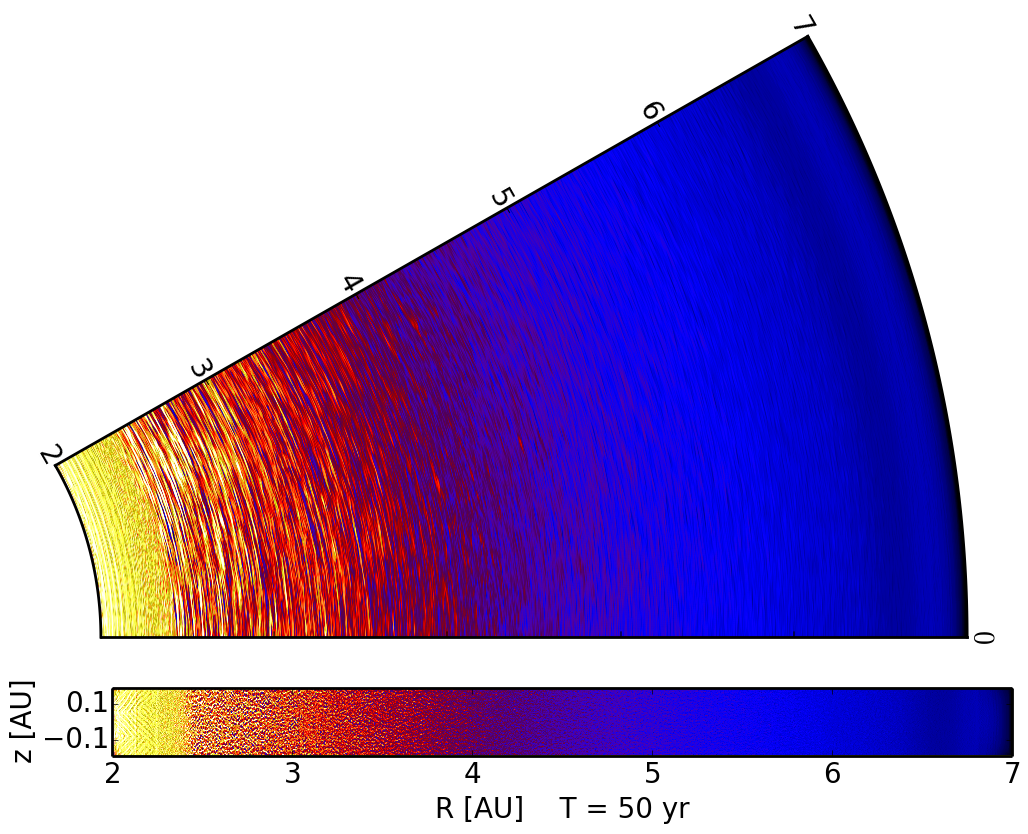
\includegraphics[width=0.44\linewidth]{figures/slice_sg_01}
   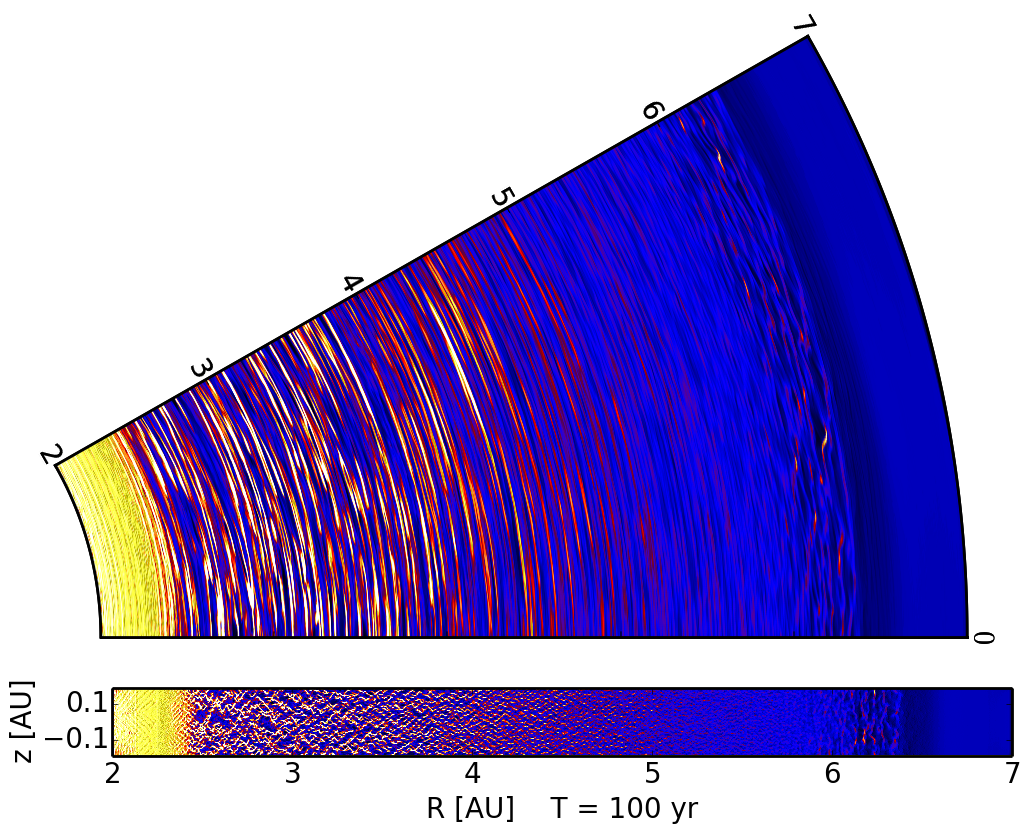
\includegraphics[width=0.44\linewidth]{figures/slice_sg_02} \\
   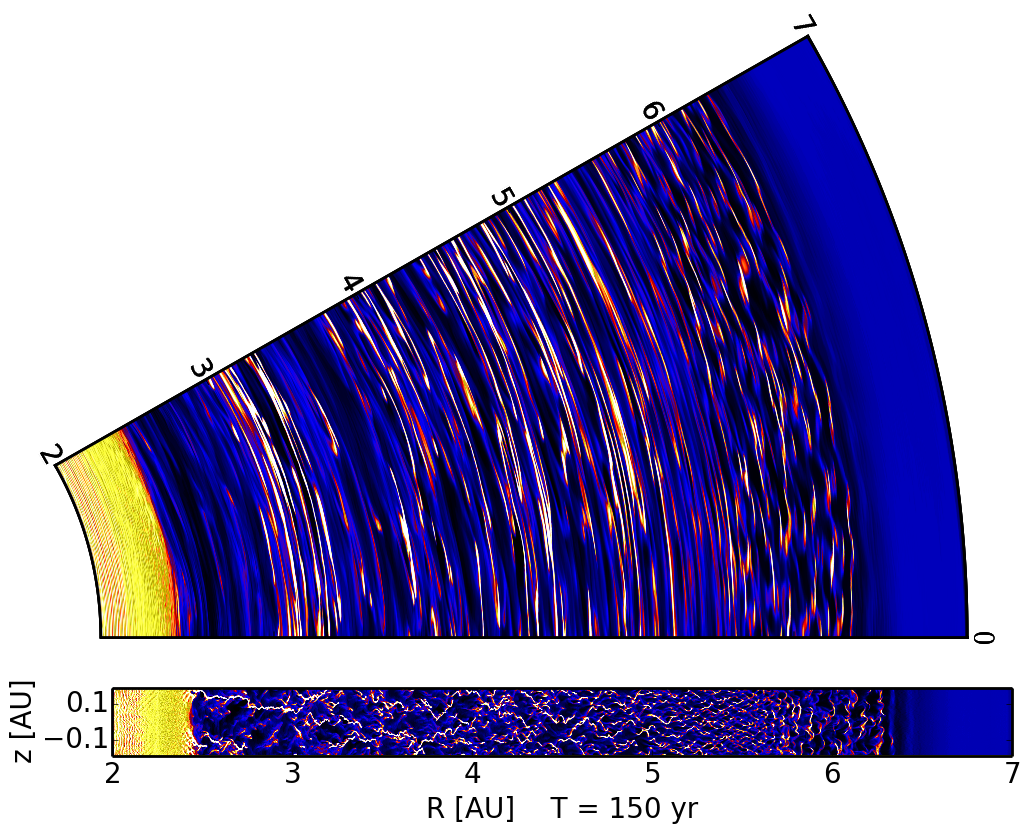
\includegraphics[width=0.44\linewidth]{figures/slice_sg_03}
   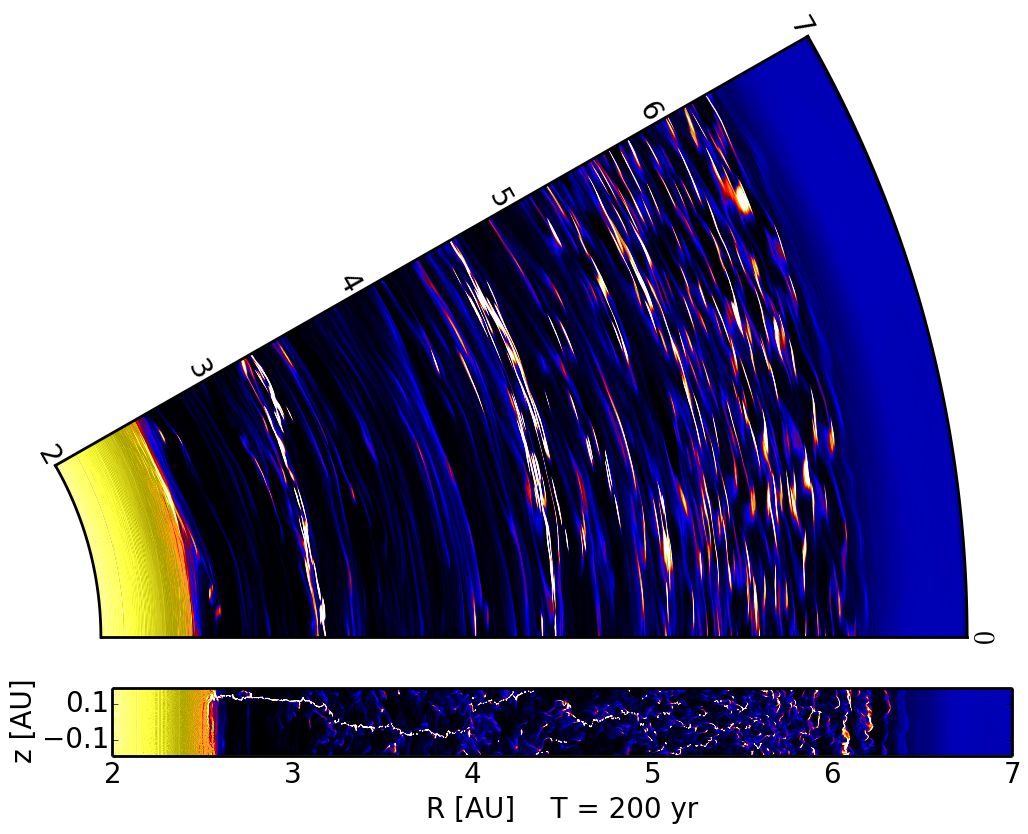
\includegraphics[width=0.44\linewidth]{figures/slice_sg_04} \\
   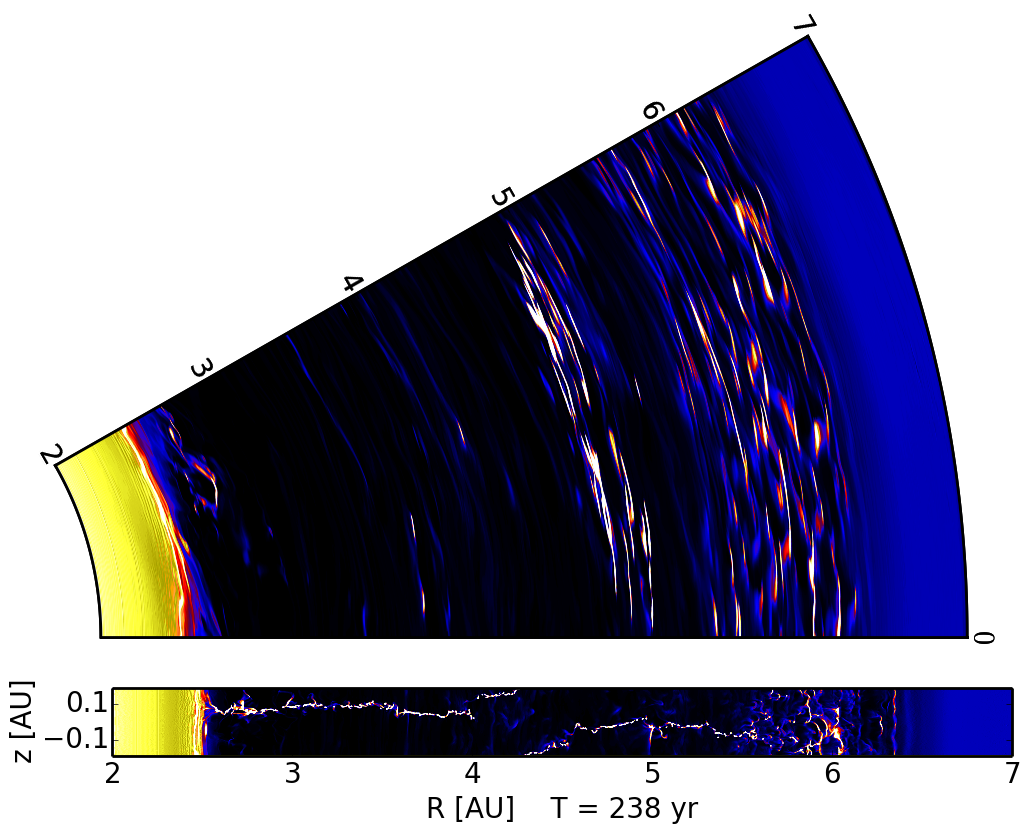
\includegraphics[width=0.44\linewidth]{figures/slice_sg_05}
   \caption{
      Migawki z symulacji BD3dS obrazujące gęstość pyłu w cięciach w
      płaszczyznach $R -\varphi$ oraz $R - z$ przechodzących przez środek 
   domeny obliczeniowej, dla czasów $T= 50, 100, 150, 200, 250$}
   \label{fig:slicesg}
\end{figure}
%
\par Wpływ samograwitacji na ewolucję układu dobrze obrazuje zestawienie
histogramów masy pyłu w funkcji promienia orbitalnego i gęstości pyłu
(Rysunek~\ref{fig:hists}). Dla symulacji BD3d, po mimo osiągnięcia przez nią
lokalnie zagęszczeń o $1\div1.5$ rzędów większych niż początkowy rozkład,
większość masy pyłu jest równomiernie rozłożona pomiędzy gęstościami $10^{-11}
\div 5\cdot10^{-10}\g\cm^{-3}$. W połączeniu obrazem wyłaniającym się z cięć
przez domenę obliczeniową, sugeruje to krótki czas życia zagęszczeń i
nieustający przepływ masy pomiędzy obszarami o niskiej i wysokiej gęstości.
Natomiast w symulacji BD3dS rozkład masy jest zgoła inny. Po osiągnięciu
granicznej wartości gęstości $\sim10^{-9}\g\cm^{-3}$ masa zaczyna ,,uciekać'' w
kierunku maksymalnej gęstości. Wytwarza się rozkład potęgowy opadający w
kierunku rzadszych obszarów, z wyraźnym gwałtownym obcięciem na wartości
granicznej gęstości $\sim10^{-8}\g\cm^{-3}$.
%
\begin{figure} 
  \centering
  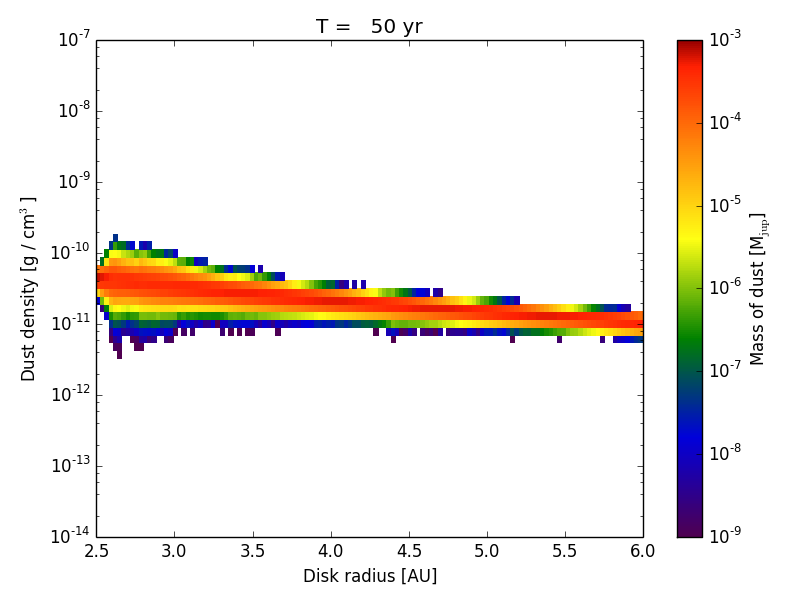
\includegraphics[width=0.4\linewidth]{figures/hist2d_nosg_01.png}
  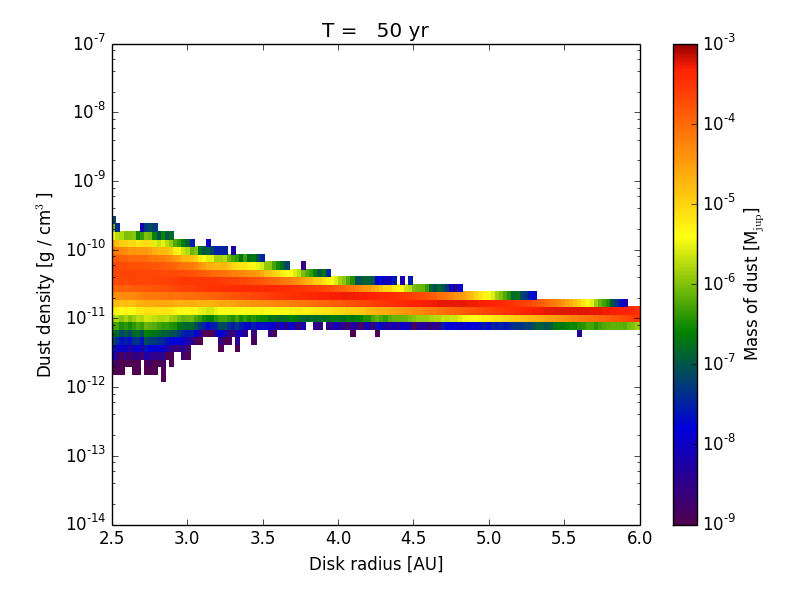
\includegraphics[width=0.4\linewidth]{figures/hist2d_sg_01.png} \\
  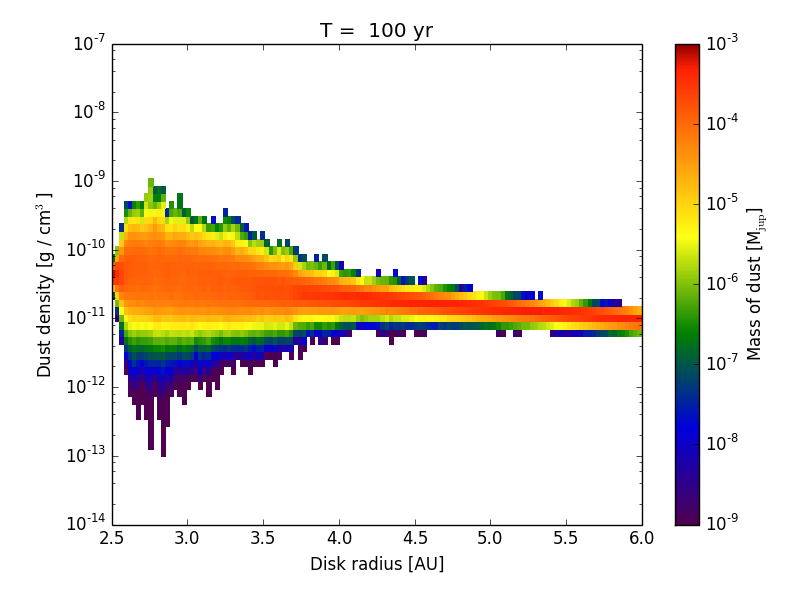
\includegraphics[width=0.4\linewidth]{figures/hist2d_nosg_02.png}
  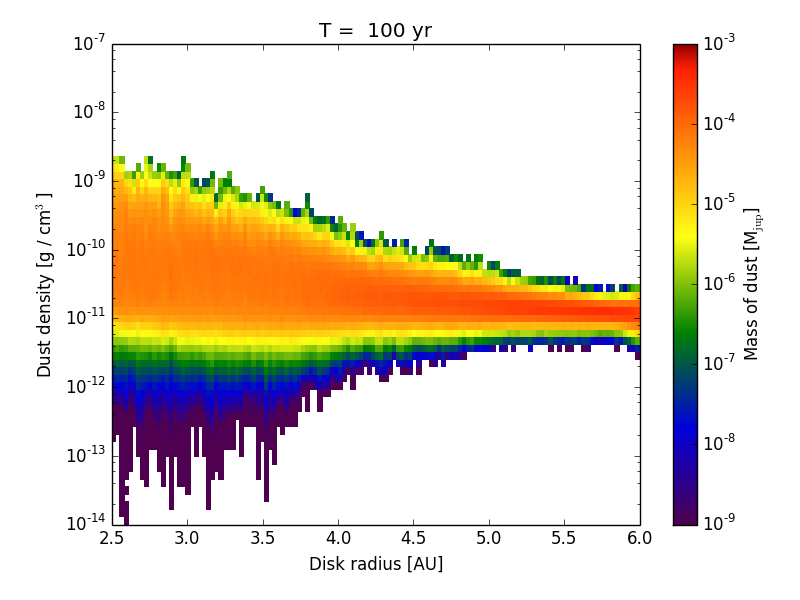
\includegraphics[width=0.4\linewidth]{figures/hist2d_sg_02.png} \\
  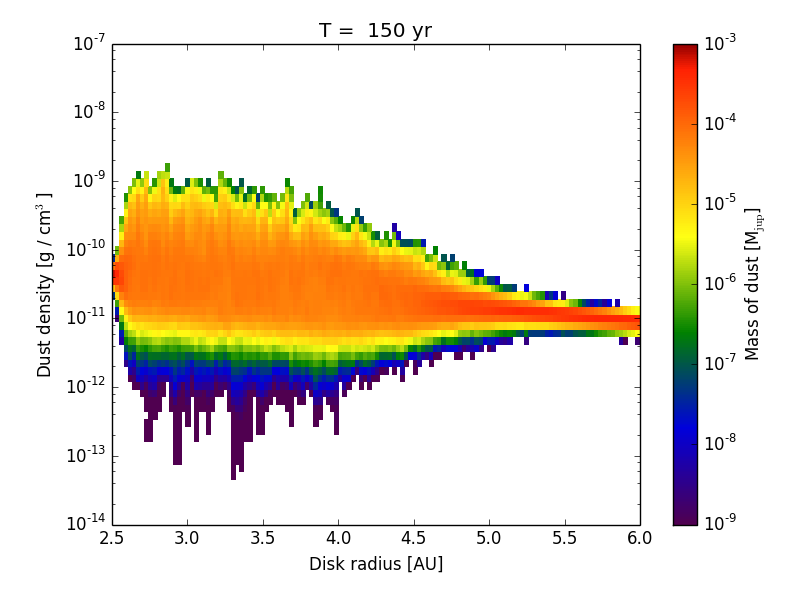
\includegraphics[width=0.4\linewidth]{figures/hist2d_nosg_03.png}
  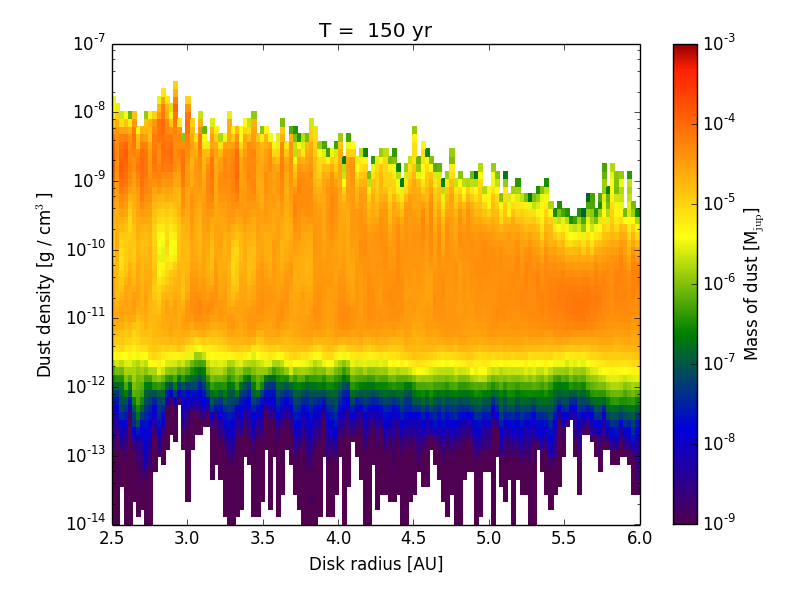
\includegraphics[width=0.4\linewidth]{figures/hist2d_sg_03.png} \\
  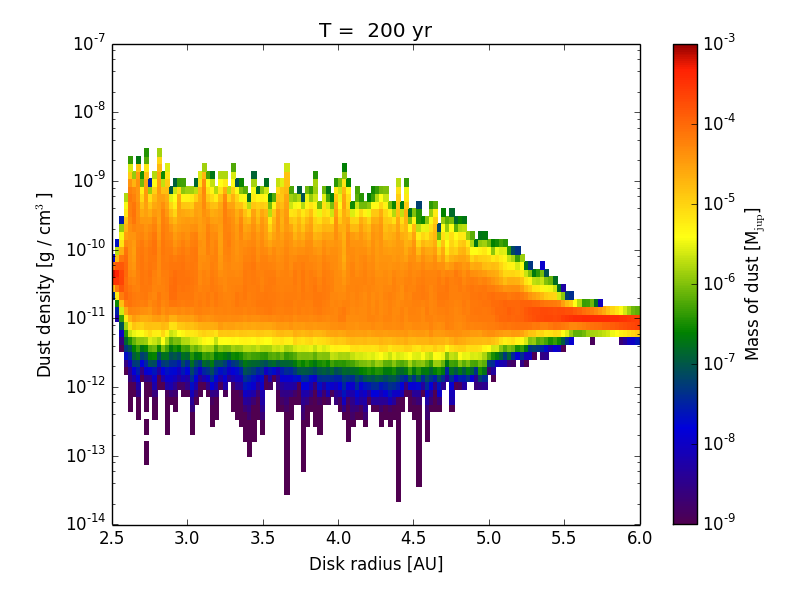
\includegraphics[width=0.4\linewidth]{figures/hist2d_nosg_04.png}
  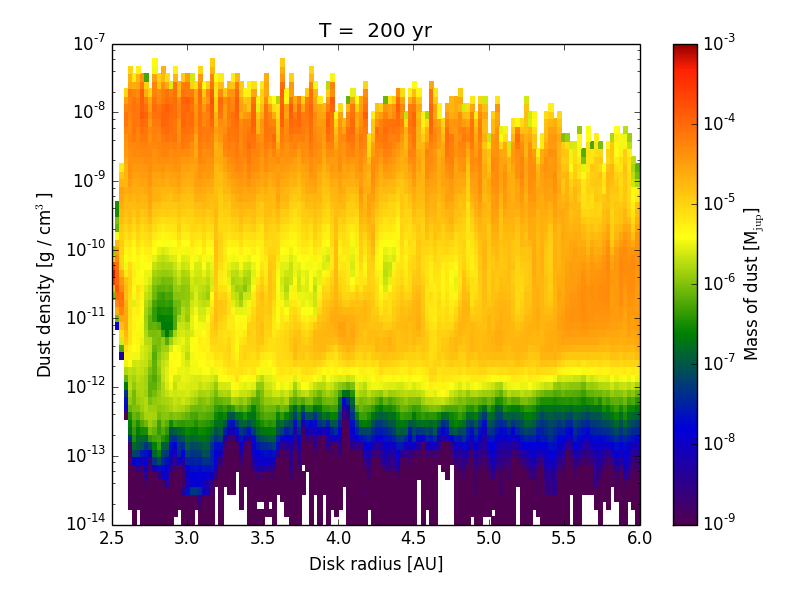
\includegraphics[width=0.4\linewidth]{figures/hist2d_sg_04.png} 
  \caption{Histogramy masy pyłu w funkcji promienia i gęstości pyłu, lewa
  kolumna bez samograwitacji, prawa kolumna z samograwitacja}
  \label{fig:hists} 
\end{figure}
%
\par Histogram masy niestety nie daję informacji o kształcie i
charakterystycznych skalach obiektów w których znajduje się większość masy pyłu,
ani nie pozwala stwierdzić czy pył jest grawitacyjnie związany. W celu
rozszerzenia przeprowadzonej analizy zebrany materiał poddano procedurze
identyfikacji topologicznie powiązanych ze sobą komórek obliczeniowych
znajdujących się w przedziale gęstości $10^{-10}\div10^{-8}\g\cm^{-3}$. W tym
celu wykorzystano pakiet do analizy i wizualizacji
danych~\yt{}~\footnote{Szczegółowe informacje na temat \emph{clump-finder'a}
można znaleźć w rozdziale 7.7 w pracy~\cite{yt}. Autor niniejszej pracy
rozszerzył pakiet \yt{} o możliwość czytania plików wynikowych z kodu
PIERNIK, a także zaimplementował wsparcie dla współrzędnych cylindrycznych.}.
Uzyskanie informacji o topologii rozkładu gęstości pyłu jest pierwszym krokiem w
celu ustalenia, czy powstające zagęszczenia są w stanie utworzyć grawitacyjnie
związane obiekty. Dla każdego zidentyfikowanego obiektu -- ,,clumpu'', można
określić relację pomiędzy jego energią kinetyczną, a studnią potencjału w której
się znajduje. Kryterium związania można wyrazić przez

\begin{equation}
   \label{eq:bcrit}
   E_{\textrm{kin}} \equiv \sum\limits_{i=1}^N \frac{m_i\tilde{\mathbf{v}}_i^2}{2} 
   < \sum\limits_{i=1}^N m_i\tilde{\Phi}_i \equiv E_{\textrm{pot}},
\end{equation}
gdzie $N$ to liczba komórek obliczeniowych wchodzących w skład clumpu, $m_i$,
$\tilde{\mathbf{v}}$, $\Phi_i$ to odpowiednio masa pyłu, prędkość w układzie
środka masy clumpu, potencjał wynikający z samograwitacji w poszczególnej
komórce. Potencjał samograwitacyjny został uzyskany bezpośrednio z PIERNIKa jako
rozwiązanie równania Poissona~\mref{eq:poisson} dla gęstości sumarycznej obu
składników płynowych. Ze względu na gładki rozkład gęstości gazu, jego
kontrybucję można było wyeliminować poprzez odjęcie od potencjału
samograwitacyjnego w każdej komórce obliczeniowej wartości średniej z tego
potencjału dla każdej orbity
\begin{equation}
   \tilde{\Phi}_i(R,\varphi,z) = \Phi_i(R,\varphi,z) -
   \left<\Phi_i\right>_{z\varphi}(R).
\end{equation}
%
Przy obliczaniu energii kinetycznej clumpu, poza przejściem z prędkością do układu środka
masy w celu uwzględnienia wpływu rotacji obłoku na jego kontrakcję, dodatkowo
wzięto pod uwagę możliwy wpływ turbulencji, która nie jest opisywana przyjętym
modelem
\begin{equation}
   \label{eq:ekin}
   \tilde{\mathbf{v}}_i = \mathbf{v}_i - \frac{\sum m_i \mathbf{v}_i}{\sum m_i}
   + \alpha c_s^2,
\end{equation}
gdzie wartość $\alpha$ ustalono na $0.05$. Zastosowanie
kryterium~\mref{eq:bcrit} dla każdego zidentyfikowanego obiektu, pozwoliło na
oszacowanie że ok. $19\%$ masy pyłu po czasie $T = 250\yr$ skupiła się w formie
grawitacyjnie związanych obłoków. Na wynik ten ma wpływ dobór parametru $\alpha$
ze względu na postać równania energii kinetycznej~\mref{eq:ekin}. Dla $\alpha <
0.05$ wyraz wynikający z turbulentnego transportu momentu pędu staje się
zaniedbywalny i nie zmienia liczby związanych obłoków pyłu. Dla $\alpha = 0.1$
związana masa pyłu spada do $\sim 9\%$ całkowitej masy.  Szczegółowy histogram
mas wszystkich zidentyfikowanych obiektów ($\alpha = 0.05$) został przedstawiony
na Rysunku~\ref{fig:masshist}.

\begin{figure}
   \centering
   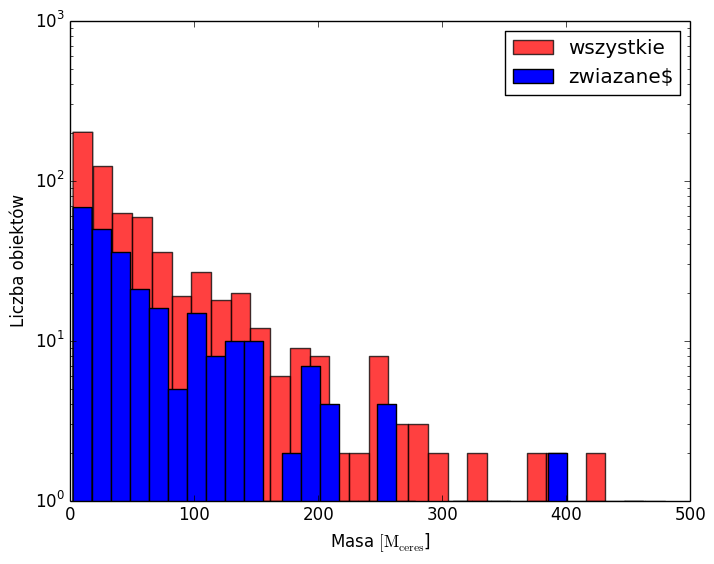
\includegraphics[width=0.49\linewidth]{figures/masshist.png}
   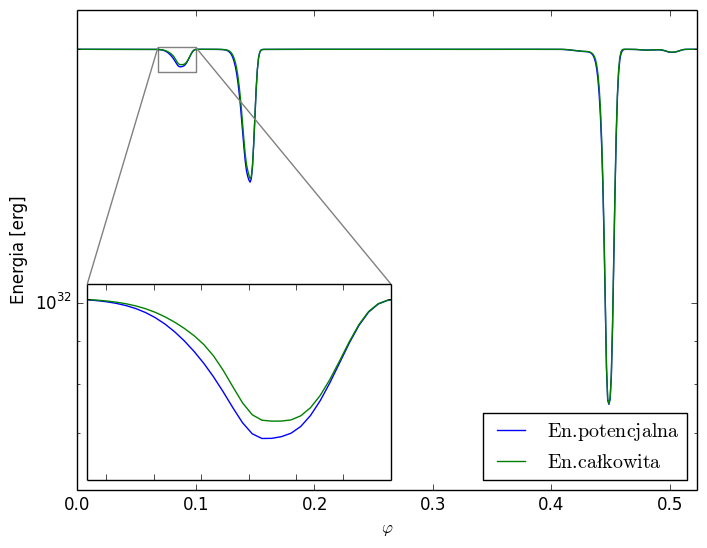
\includegraphics[width=0.49\linewidth]{figures/energie.png}
   \caption{(Lewy panel) Histogram przedstawiający rozkład masy w topologicznie powiązanych
   obiektach istniejących w domenie obliczeniowej dla symulacji BD3dS dla czasu
   $T=250\yr$. Kolorem niebieskim zaznaczono clumpy związane grawitacyjnie, zaś
   kolorem czerwonym wszystkie obiekty.
   (Prawy panel) Przekrój azymutalny przez domenę obliczeniową dla $R=3.84\AU$
   i $z=0.01\AU$ dla czasu $T=250\yr$ pokazujący energię potencjalną (zgodnie z
   definicją w równaniu~\mref{eq:bcrit}) oraz sumę energii potencjalnej i energii
   kinetycznej dla danego clumpu.}
   \label{fig:masshist}
\end{figure}
%
\begin{figure}
   \centering
   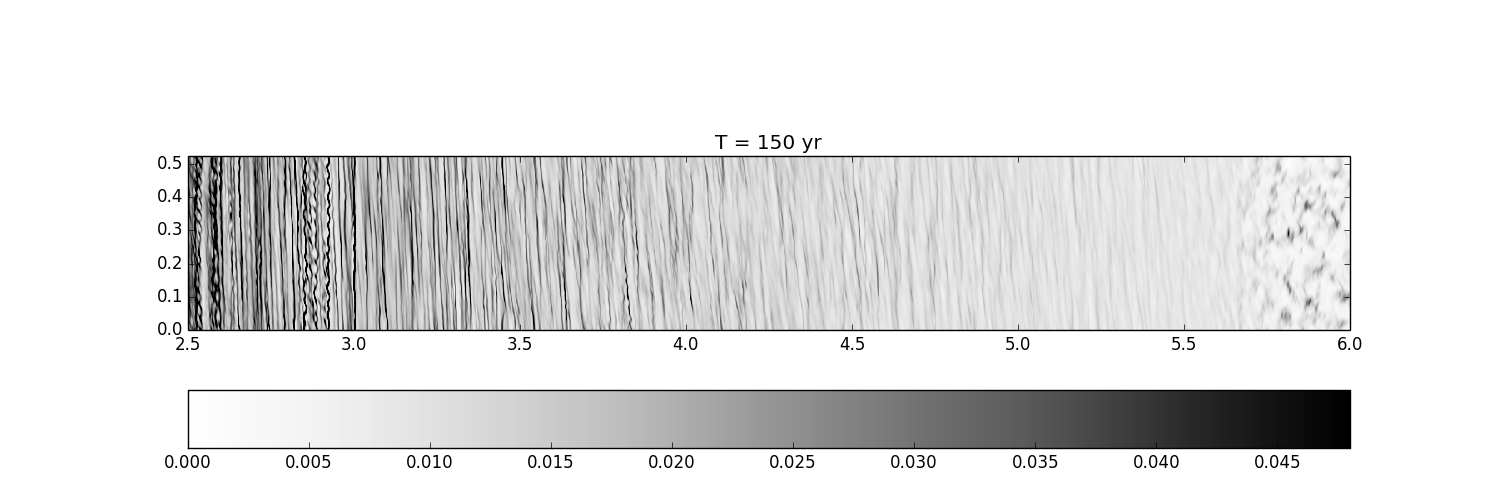
\includegraphics[width=0.95\linewidth]{figures/proj1.png}\\
   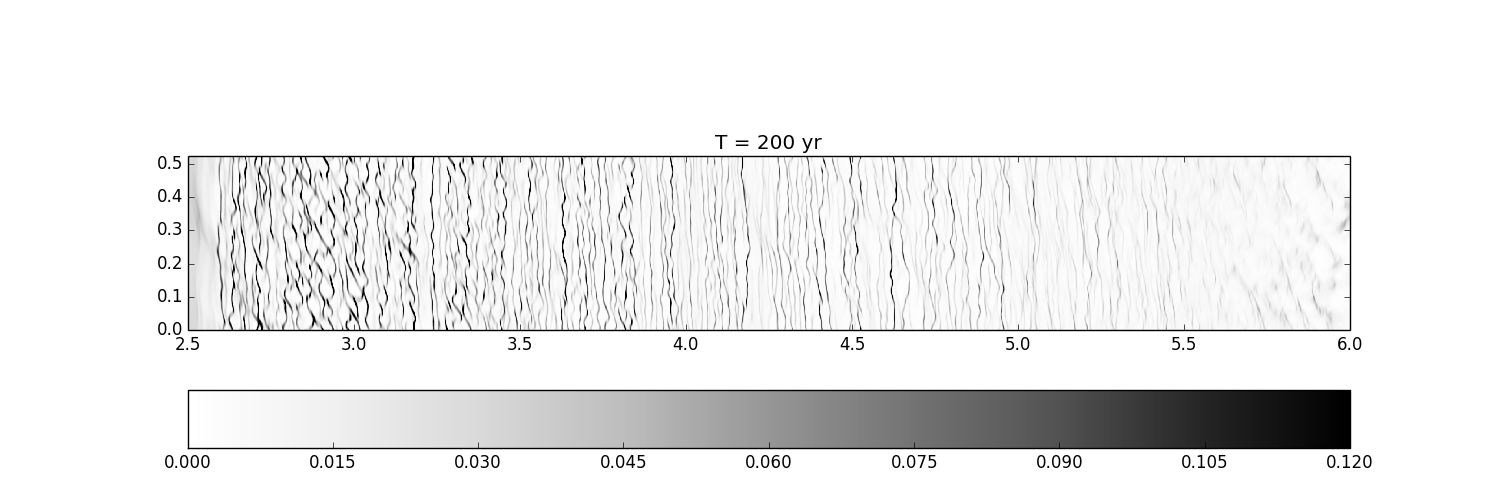
\includegraphics[width=0.95\linewidth]{figures/proj2.png}\\
   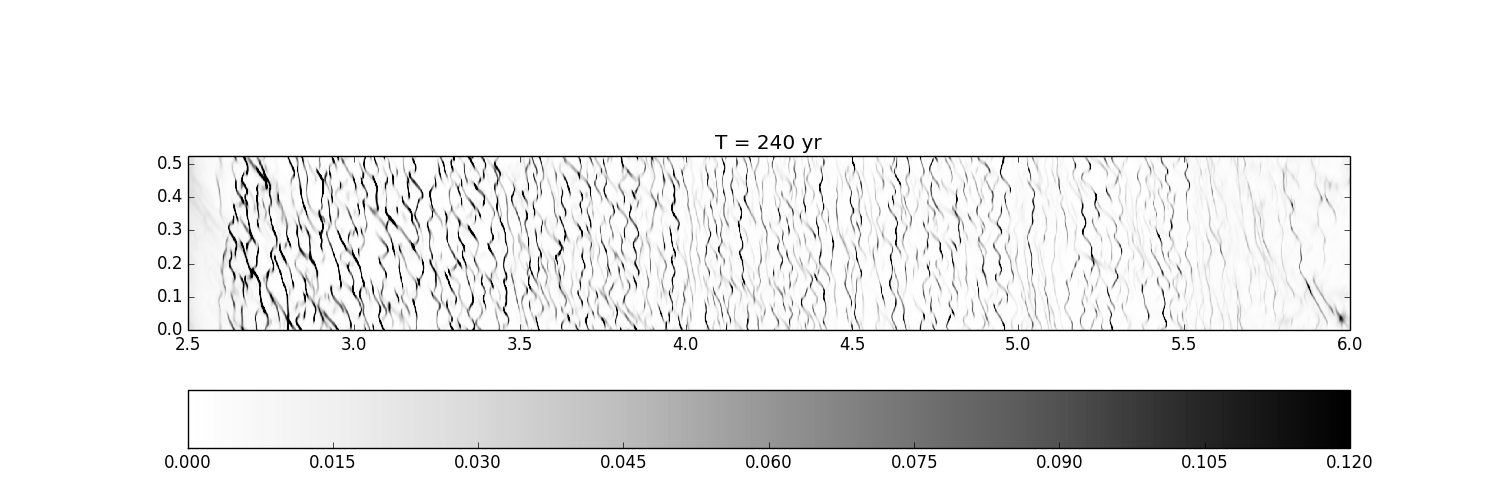
\includegraphics[width=0.95\linewidth]{figures/proj3.png}
   \caption{Gęstość
      kolumnowa pyłu w symulacji BD3dS dla czasu $T=150, 200, 250\yr$}
   \label{fig:projs}
\end{figure}
%
\begin{figure}
   \centering
   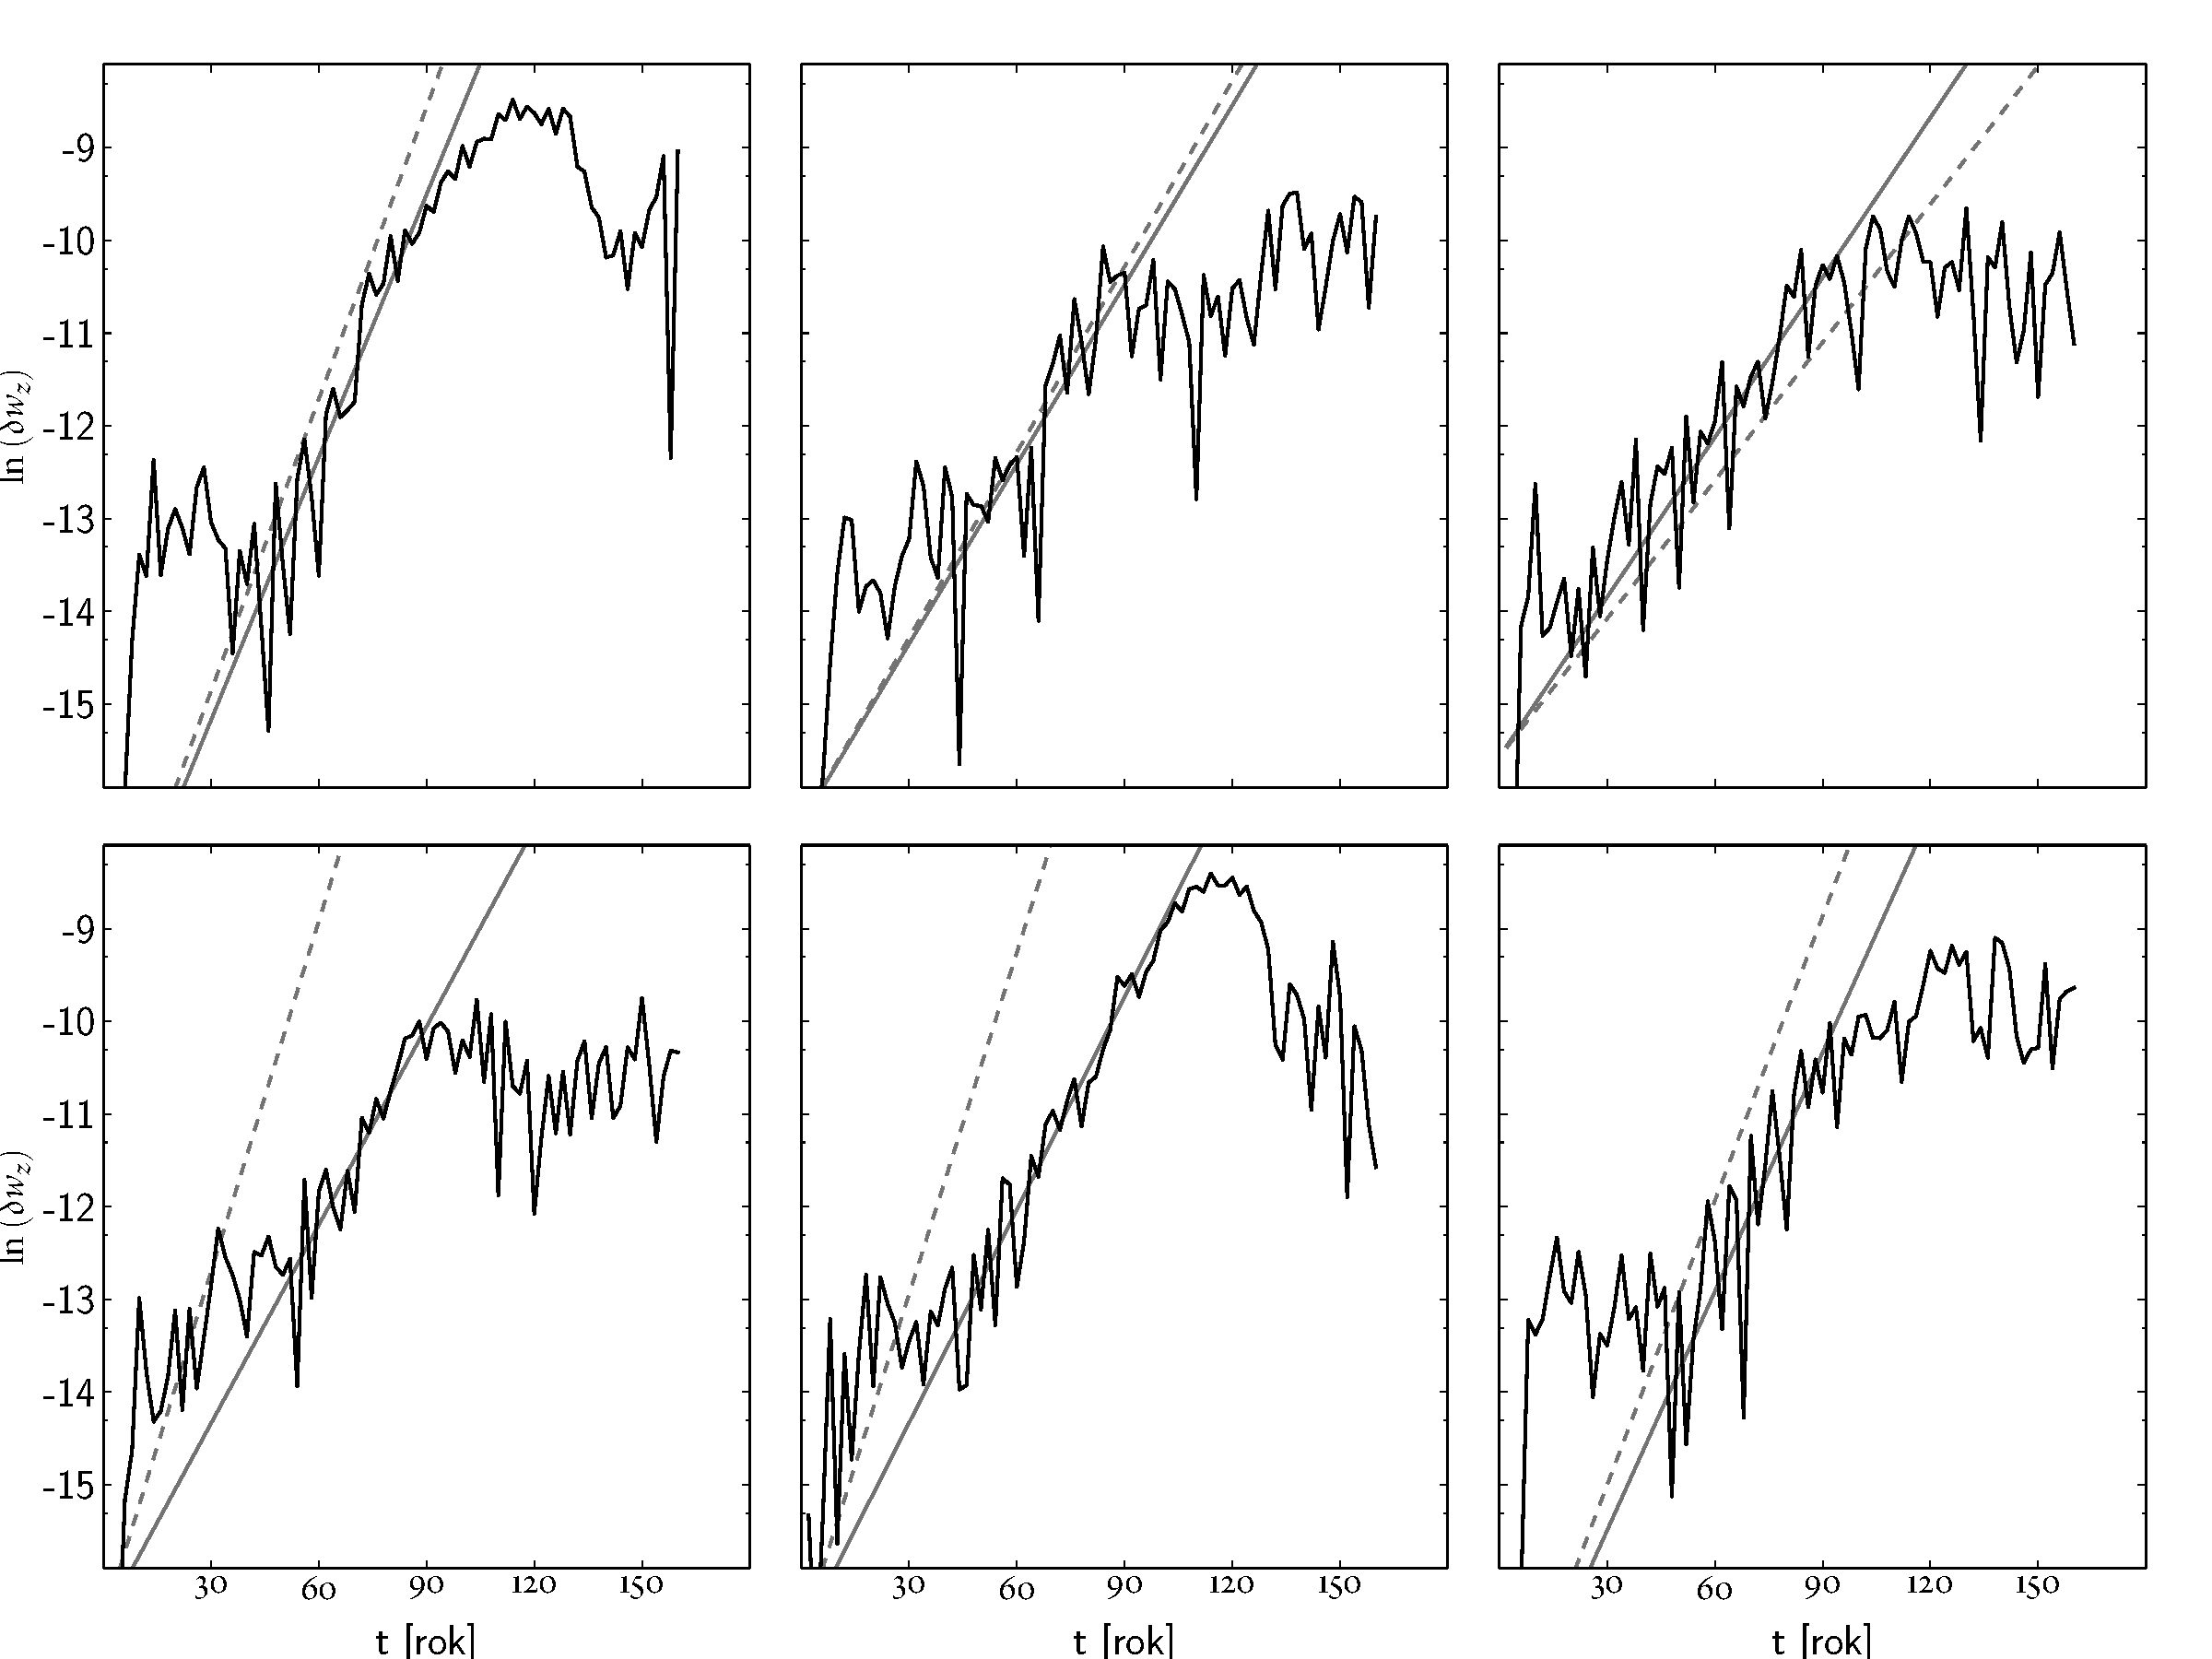
\includegraphics[width=0.95\linewidth]{figures/nosg_vlzd_growth}
   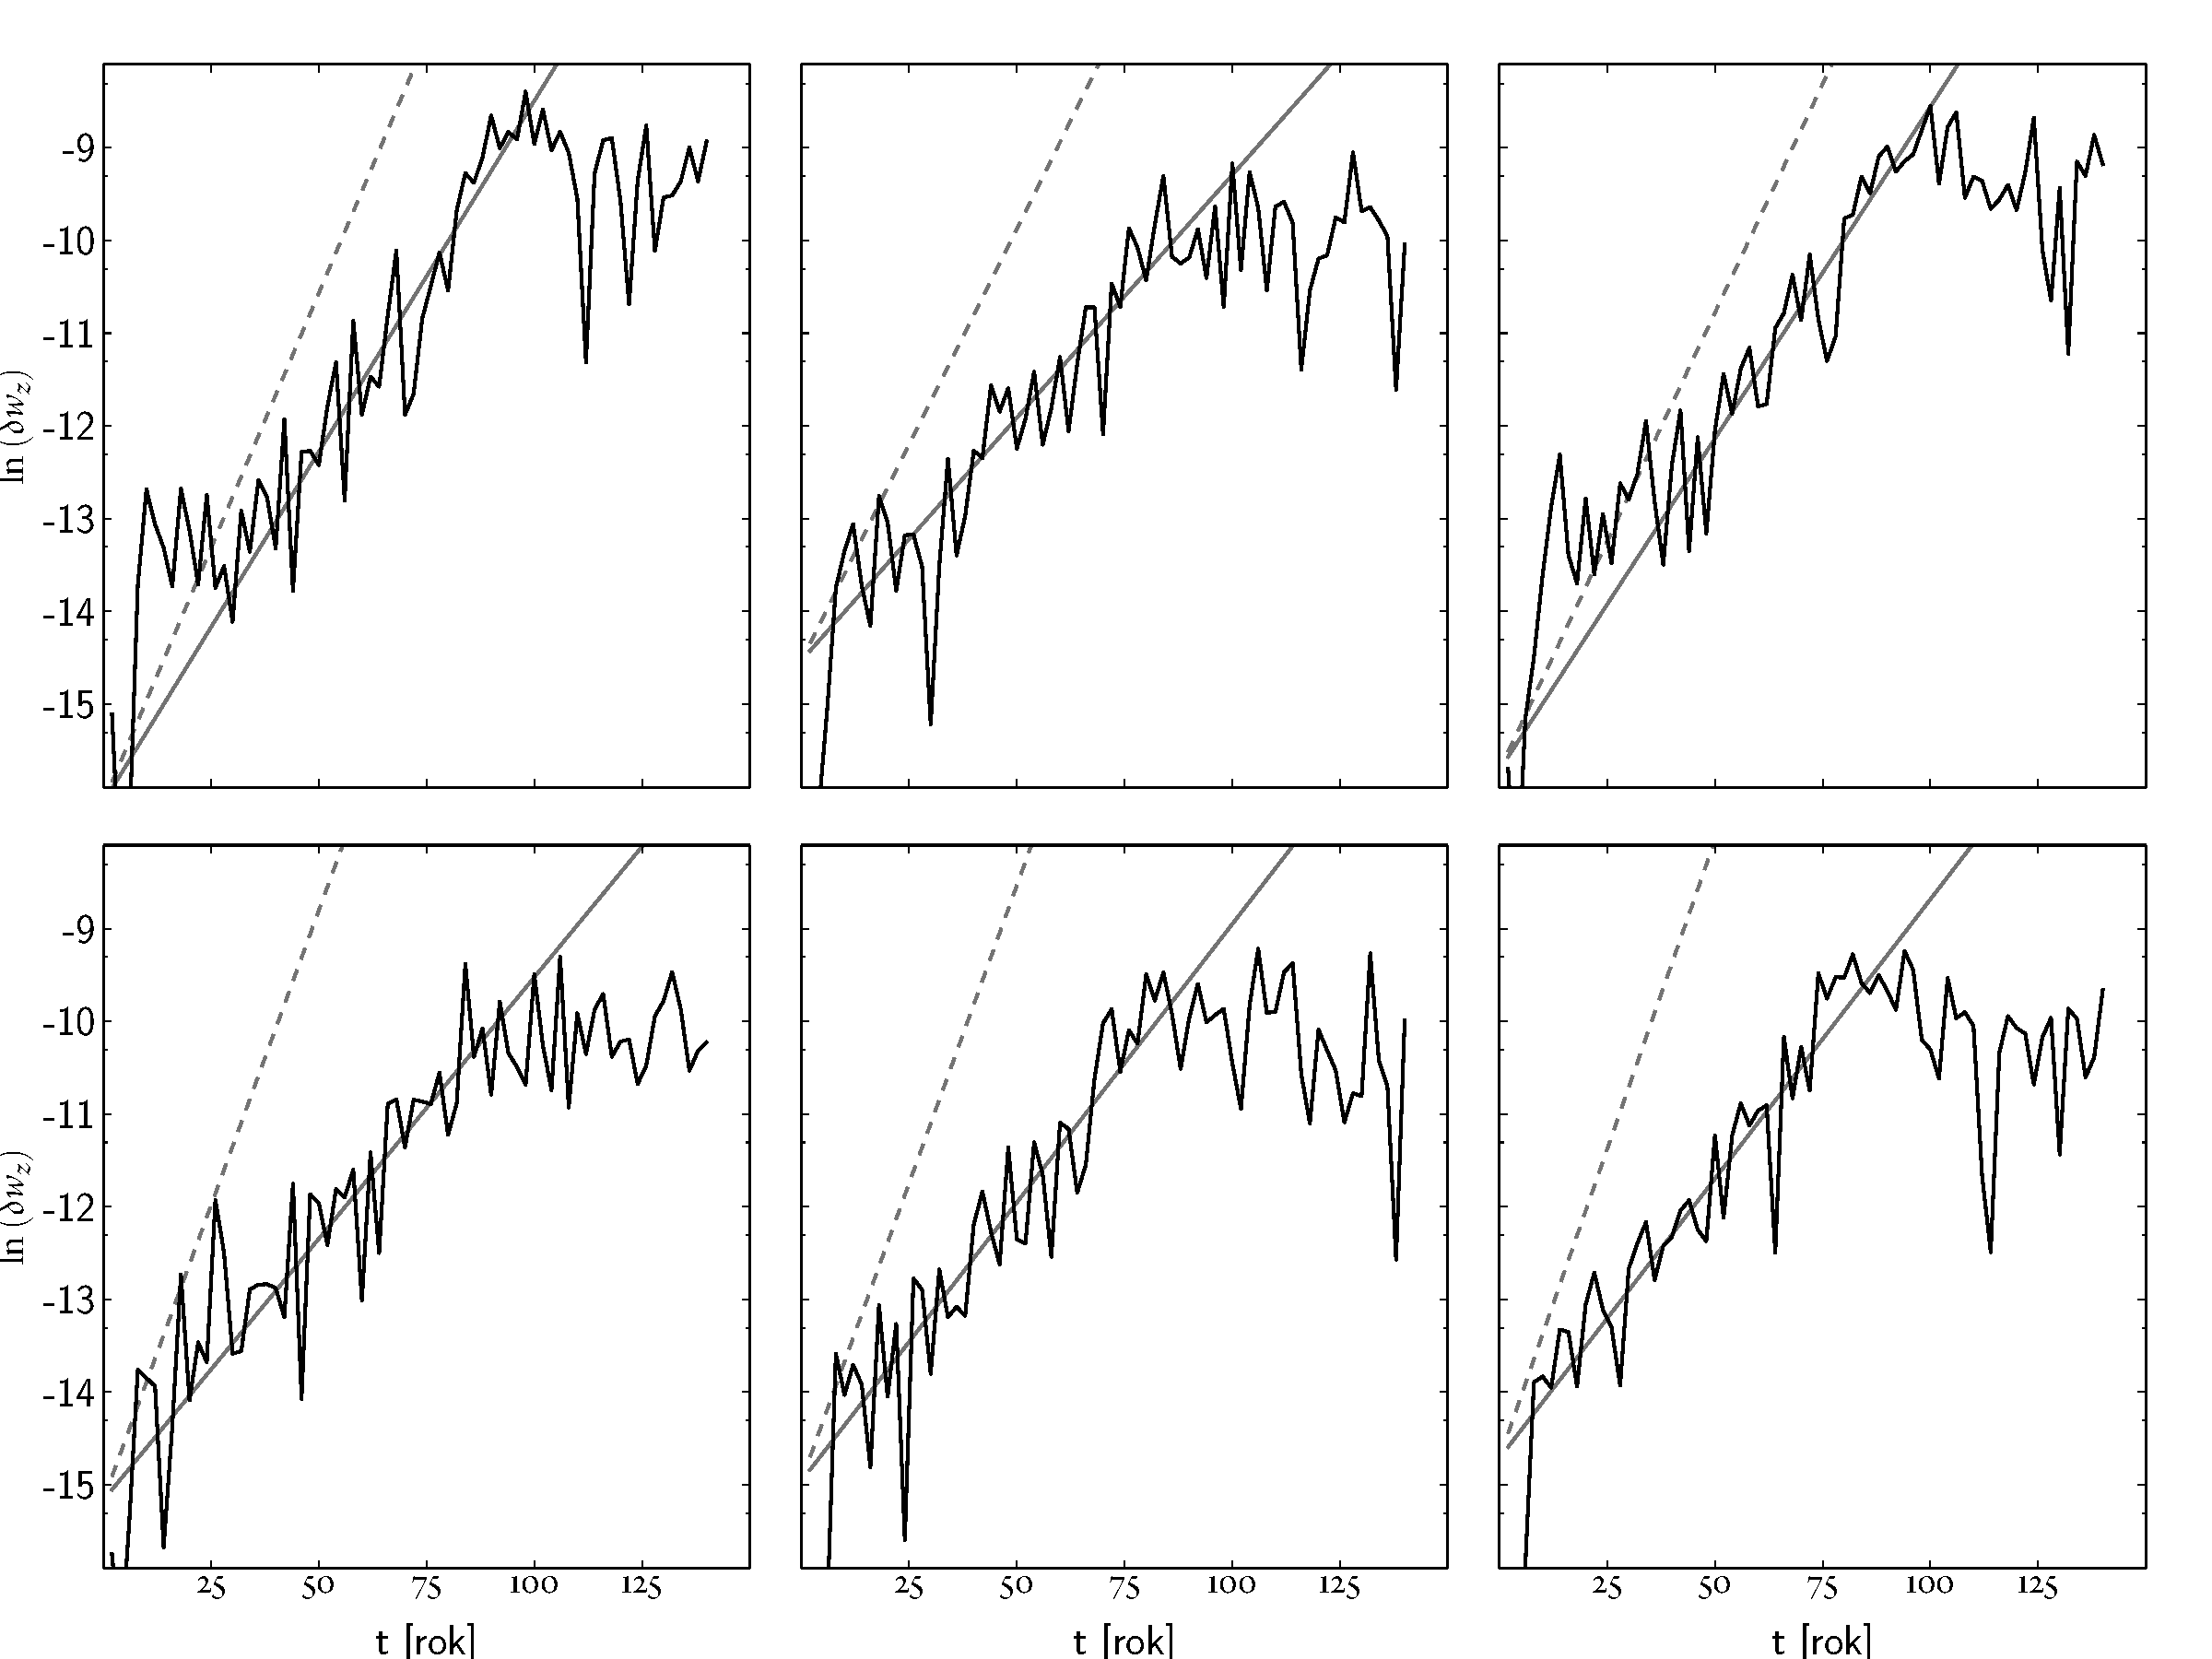
\includegraphics[width=0.95\linewidth]{figures/sg_vlzd_growth}
   \caption{6 dominujacych modów z BD3d i BD3dS}
   \label{fig:modes3d}
\end{figure}
%   
\begin{figure}
   \centering
   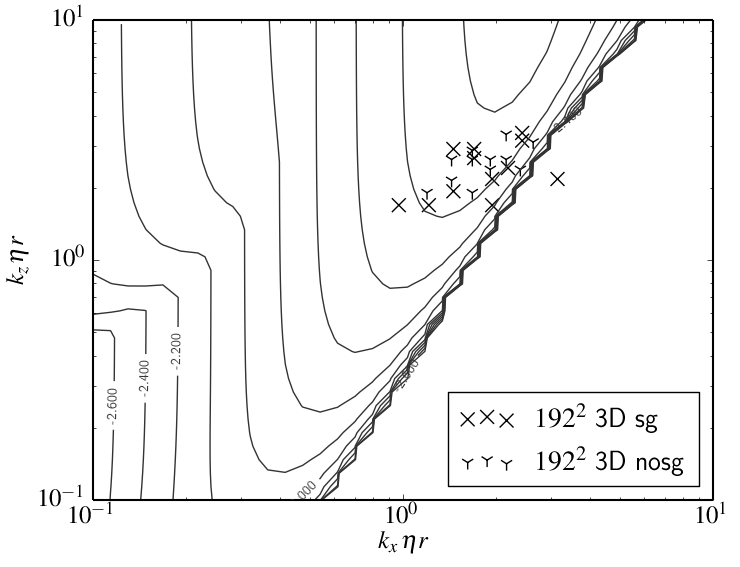
\includegraphics[width=0.5\linewidth]{figures/3d_map_x3_50.png}
   \caption{Mapa stabilności BD3d i BD3dS}
   \label{fig:map3d}
\end{figure}
% x3_50n.png
% vim: tw=80 ts=3: 
